% ICE: Infinite Context Engine — Research Paper
% Generic, venue-agnostic academic format (no conference-specific class required).
% Self-contained — no external files required for compilation.
% Once you pick a target venue, swap this preamble for that venue's template;
% the body content (sections, tables, references) will carry over unchanged.
%
%=====================================================================
% ⚑ THIS IS THE CANONICAL WORKING FILE. Substantive edits happen HERE.
%
% ⚑ "v2" IN THIS FILENAME IS A PAPER DRAFT NUMBER, *NOT* A SYSTEM VERSION.
%   CLAUDE.md's v1/v2/v3 are SYSTEM versions. This file's "v2" means
%   "paper draft 2" (the post-TMLR-desk-reject reframe). The two scales
%   collide on the same token and MUST NEVER be read across.
%   It happens to REPORT system v2 (git tag `v2-paper-eval`) — that is a
%   coincidence of history, not what the filename means.
%
% ⚑ THERE IS NO `ICE_paper_v3` AND THERE MUST NEVER BE ONE. A future
%   session would read "paper v3" as "the paper about system v3", which is
%   false: this paper reports system-v2 numbers and will continue to, even
%   as v3 work lands on main.
%
% ⚑ DO NOT RENAME THIS FILE. `ICE_paper_v2.pdf` is a PUBLISHED URL —
%   README.md:153 links it, and it was sent to an external researcher in
%   endorsement correspondence. Renaming breaks a live external link.
%
% Sibling files: `ICE_paper_tist.tex` is the FROZEN record of what ACM TIST
% received (rejected 2026-08-28); `ICE_paper_tmlr.tex` / `ICE_paper_v2_tmlr.tex`
% are the frozen TMLR submissions. None of those take new edits.
%=====================================================================

\documentclass[11pt,a4paper]{article}

% --- Page geometry: comfortable single-column layout ---
\usepackage[margin=1in]{geometry}

\usepackage{booktabs}
\usepackage{multirow}
\usepackage{amsmath}
\usepackage{amssymb}
\usepackage{graphicx}
\usepackage{xcolor}
\usepackage{enumitem}
\usepackage{microtype}
\usepackage{url}
\usepackage[htt]{hyphenat} % allow hyphenation of \texttt{} content (long code identifiers)
\sloppy
\tolerance=2000
\emergencystretch=3em
\usepackage[round,authoryear,sort]{natbib}
\usepackage[colorlinks=true,linkcolor=blue!50!black,citecolor=blue!50!black,urlcolor=blue!50!black]{hyperref}
\usepackage{cleveref}
\usepackage{caption}
\usepackage{array}
\usepackage{ragged2e}
\usepackage{pgfplots}
\pgfplotsset{compat=1.18}
\usetikzlibrary{patterns,arrows.meta,positioning,fit,backgrounds,calc}

% --- Shared styles for the architecture diagrams ---
\tikzset{
  icebox/.style={draw=blue!40!black, fill=blue!5, rounded corners=2pt,
    align=center, font=\scriptsize, inner sep=3pt, minimum height=6mm},
  icephase/.style={draw=gray!50, fill=gray!8, rounded corners=3pt,
    align=center, font=\scriptsize\bfseries, inner sep=4pt},
  icestore/.style={draw=teal!50!black, fill=teal!8, rounded corners=2pt,
    align=center, font=\scriptsize, inner sep=3pt, minimum width=17mm, minimum height=9mm},
  iceleg/.style={draw=orange!60!black, fill=orange!8, rounded corners=2pt,
    align=center, font=\scriptsize, inner sep=2pt, minimum width=15mm, minimum height=6mm},
  icecore/.style={draw=red!50!black, fill=red!6, rounded corners=2pt,
    align=center, font=\scriptsize\bfseries, inner sep=3pt},
  iceflow/.style={-{Stealth[length=2mm]}, draw=gray!60, thick},
  iceflowd/.style={-{Stealth[length=2mm]}, draw=gray!60, thick, dashed},
}

% --- Table helpers ---
\newcolumntype{L}[1]{>{\raggedright\arraybackslash}p{#1}}
\newcolumntype{C}[1]{>{\centering\arraybackslash}p{#1}}
\newcolumntype{R}[1]{>{\raggedleft\arraybackslash}p{#1}}

% --- Section spacing (compact, journal-article feel) ---
\usepackage{titlesec}
\titlespacing*{\section}{0pt}{1.4em}{0.7em}
\titlespacing*{\subsection}{0pt}{1.1em}{0.5em}

\setlength{\textfloatsep}{10pt plus 2pt minus 2pt}
\setlength{\intextsep}{8pt plus 2pt minus 2pt}

% --- Float placement: let floats fill more of a page and drift less far ---
\renewcommand{\topfraction}{0.9}
\renewcommand{\bottomfraction}{0.8}
\renewcommand{\textfraction}{0.07}
\renewcommand{\floatpagefraction}{0.7}
\setcounter{topnumber}{3}
\setcounter{bottomnumber}{2}
\setcounter{totalnumber}{5}
\renewcommand{\arraystretch}{1.15}
\captionsetup{font=small,labelfont=bf}

\title{\bfseries LSREP: A Longitudinal State-Replay Protocol for Evaluating Conversational Memory, with ICE as a Local-First System Under Test}

\author{Deepesh Sonar\\[2pt]
  \normalsize Thakur College of Engineering and Technology, Computer Engineering, Mumbai, India\\
  \normalsize\texttt{18deepnar@gmail.com}}

\date{}

\begin{document}
\maketitle
\thispagestyle{empty}

\begin{abstract}
Conversational memory systems accumulate, decay, and revise state, yet fixed-history benchmarks observe retrieval at one endpoint rather than those dynamics. We introduce \textbf{LSREP}, a Longitudinal State-Replay Evaluation Protocol that reconstructs memory at successive checkpoints and scores against evolving ground truth. ICE, a local-first multi-store memory middleware, serves as the system under test. Across 1{,}985 turns, 1{,}211 probes, and 50 checkpoints, ICE ties a vector-RAG baseline on answer quality (paired $\Delta=+0.00$, 95\% CI $[-0.07,+0.07]$) while injecting 32\% fewer fragments and winning more blind comparisons (30.6\% vs.\ 21.2\%). Under extreme per-turn density, the unbudgeted baseline fails on 94.2\% of probes while ICE holds a mean score of 4.33. A fidelity audit nevertheless finds one defective component, several unexercised components, and a result carried principally by episodic retrieval, rank fusion, prompt assembly, and the token budget. We then test transfer on all 500 questions of LongMemEval's public evidence-only oracle condition. With the official decision prompts but a local Gemma-4 12B judge, fresh-session ICE v2 scores 55.2\% over 478 obtainable verdicts (all-case bounds 52.8--57.2\%) against vector-RAG's 80.2\% (77.6--80.8\%): ICE has higher point estimates on abstention and preference but fails sharply on multi-session and temporal reasoning. We stop before distractor-heavy LongMemEval-S because the evidence-only prerequisite already rejects cross-conversation effectiveness. The combined evidence therefore separates within-conversation success from fresh-session failure, and ``did not help'' from ``did not run''---distinctions an aggregate score alone conceals.
\end{abstract}


%======================================================================
\section{Introduction}
\label{sec:intro}

Absent an explicit persistence layer, a language model can use only what remains in its current context. Enlarging that context does not make every token equally usable: models attend unevenly across long inputs and degrade on information away from their edges~\citep{liu2024lost}, while effective context is often shorter than the advertised limit~\citep{hsieh2024ruler}. Commercial assistants now provide cross-session memory, so literal session-level amnesia is no longer a universal description. The open questions are instead what is retained, how revisions and forgetting are represented, and whether the user can inspect and govern the store.

Research has approached those questions through multi-session dialogue~\citep{xu2022msc,jang2023chronicles}, long-history benchmarks~\citep{maharana2024locomo,wu2025longmemeval}, and personalised adaptation~\citep{salemi2024lamp}. These instruments accurately test whether a system can answer from a supplied history. They do not, by design, observe a deployed memory state repeatedly accumulating, decaying, being reinforced, and replacing superseded beliefs between questions.

The Infinite Context Engine (ICE) is a local-first middleware around an otherwise stateless answering model. It stores episodic turns, a temporally-versioned knowledge graph, procedural patterns, documents, and user-controlled memory slots; classifies each prompt; retrieves and fuses candidates; and assembles a bounded context. Externalising memory preserves it when the answering model changes and makes the store inspectable. ICE is the case study here, not the definition of the evaluation problem.

That evaluation problem is longitudinal. A system may retrieve well at one endpoint while failing to update an old fact, may appear efficient only because a component never ran, or may work inside one continuing conversation but fail when a fresh session must aggregate earlier ones. We therefore introduce LSREP alongside, rather than in place of, fixed-history benchmarks. It reconstructs state at successive checkpoints and allows the reference answer itself to evolve.

This paper makes three contributions.

\begin{enumerate}[leftmargin=*]
  \item \textbf{LSREP}, the primary contribution: a system-agnostic protocol for replaying conversational history, reconstructing state at successive checkpoints, and scoring against evolving ground truth. It is portable to another user's exported history, while the private corpus used here is not independently reproducible.
  \item \textbf{ICE as a released system under test}: a local-first multi-store architecture with intent-driven retrieval, access-weighted decay, weighted rank fusion, and a per-query token budget. The evaluated snapshot is fixed at tag \texttt{v2-paper-eval}.
  \item \textbf{A two-regime evaluation with a fidelity audit}: LSREP measures within-conversation longitudinal behaviour and a density stress case; the public LongMemEval oracle condition probes fresh-session aggregation. Their disagreement is itself a result. A component audit separately identifies defective, unexercised, contributing, and genuinely neutral mechanisms.
\end{enumerate}

The methodological claim is deliberately falsifiable: a near-zero ablation delta supports ``does not help'' only when the component is verified live and the interaction regime reaches it. We report where our own evaluation failed that standard and constrain the system claims accordingly.

%======================================================================
\section{Related Work}
\label{sec:related-work}

Prior work bearing on ICE divides along one axis: what a system assumes about the \emph{stability} of the knowledge it retrieves over time. We move along that axis, from systems that treat stored knowledge as mutable but flat (Section~\ref{sec:related-memory}), to those that give it relational structure but assume it is static (Section~\ref{sec:related-kg}), to the retrieval-augmented tradition that assumes a fixed corpus outright (Section~\ref{sec:related-rag}), then to the primitives ICE builds on (Section~\ref{sec:related-primitives}) and the benchmarks used to evaluate any of it (Section~\ref{sec:related-eval}). ICE's position is that conversational history satisfies none of the stability assumptions these lines inherit, and that its evaluation inherits the same problem. We are deliberately specific about the gaps throughout, including where a gap is one ICE does not close.

\subsection{Stateful Memory Architectures for Dialogue}
\label{sec:related-memory}

Bounded context length has driven a family of external memory hierarchies. \textbf{MemGPT}~\citep{packer2023memgpt} treats the context window as primary memory backed by unbounded external storage, paging between tiers to create the illusion of unbounded context. It is effective on short-to-medium interactions and document analysis but degrades in extended multi-session dialogue: retrieval is flat and dense, it struggles to distinguish semantically identical but contextually distinct entities over time, and it has neither a structured graph tracking entity evolution nor intent-driven routing.

\textbf{mem0}~\citep{chhikara2025mem0} targets the latency and token cost of paging with a lightweight production memory layer: a single-pass, append-only pipeline distils conversations into atomic facts, and a multi-signal retriever fuses embeddings, BM25, and entity linking, performing strongly on LoCoMo~\citep{maharana2024locomo} and LongMemEval~\citep{wu2025longmemeval} at low overhead. The cost is cognitive depth: flat key-value facts are not versioned, so contradictory or evolving facts are never systematically reconciled, and there is neither procedural memory nor a principled decay and archival mechanism.

\textbf{MemoryBank}~\citep{zhong2024memorybank} integrates an Ebbinghaus-style forgetting curve so every item carries a continuously updated strength score under time-aware decay and reinforcement, sustaining persona invariance across multi-day dialogue. It remains constrained by its retrieval substrate: no graph for associative multi-hop reasoning, and no conversation-scoped clustering. \textbf{SCMoE}~\citep{shi2024scmoe} attacks the cost of dense retrieval differently, contrasting strong and weak expert activations at inference; it optimises routing of internal representations rather than external memory, and is untested on the large, shifting per-turn documents that characterise persistent agentic memory.

Two further systems sit closer to ICE than any of the above. \textbf{HippoRAG}~\citep{gutierrez2024hipporag} builds a schemaless knowledge graph over a corpus and runs personalised PageRank across it, drawing an explicit analogy to hippocampal indexing to reach associations a flat retriever cannot; it is nonetheless indexed once over a static corpus, with no notion of a fact that is later revised. \textbf{Zep}~\citep{rasmussen2025zep} is the nearest relative of all: a temporal knowledge graph for agent memory in which edges carry validity intervals, so superseded facts are invalidated rather than overwritten. ICE shares that temporal-versioning commitment and differs on scope and siting --- Zep is a hosted service organised around a single graph, where ICE runs locally across four typed stores with intent-driven routing, a per-query token budget, and an access-weighted decay lifecycle that governs what is offered to the model at all.

Across these systems one trend recurs: static fact storage is conflated with dynamic working memory.

\textbf{Deployed commercial memory, and why it is not a baseline here.} Hosted assistants, including ChatGPT, now expose cross-session memory controls, so literal session-level amnesia is no longer a defensible description of the field. Their public interfaces, however, do not expose a memory layer that an independent evaluator can hold fixed, populate deterministically, query in isolation, and ablate separately from the answering model. Treating one as a baseline here would therefore confound its memory policy, its answering model, and its product-specific orchestration. We acknowledge these systems as deployed evidence that cross-session persistence matters, but exclude them from the controlled comparison because the mechanism under comparison is not independently observable.

\subsection{Knowledge Graphs as Dialogue Substrates}
\label{sec:related-kg}

To overcome the relational blindness of flat vector stores, several systems map text into graphs. \textbf{GraphRAG}~\citep{edge2024graphrag} answers global sense-making queries over private corpora by extracting an entity graph with a language model, partitioning it by community detection, and pre-generating hierarchical community summaries---a substantial gain in answer depth on query-focused summarisation. It assumes a temporally \emph{static} corpus: all ingested facts are equally current, and there is no versioning for an entity whose properties or relationships mutate across sessions. \textbf{KGP}~\citep{wang2023kgp} builds a graph whose nodes are passages and whose edges are semantic or lexical similarities, then deploys a traversal agent as a local navigator for multi-document question answering; \textbf{Think-on-Graph}~\citep{sun2024tog} couples the model tightly to the graph, running iterative beam search over reasoning paths and pruning irrelevant branches.

Both demonstrate the value of structural retrieval, but are tailored to single-shot question answering over static knowledge bases, treating the graph as ground-truth world knowledge. They contain no mechanism for narrative continuity, belief decay, or contradiction resolution---exactly what an evolving conversation demands. ICE borrows the topology and repurposes it for a continuously mutating conversational landscape.

\subsection{Retrieval-Augmented Generation}
\label{sec:related-rag}

\textbf{RAG}~\citep{lewis2020rag} formalised augmenting parametric knowledge with a dense index over a static corpus. Conversational history is not a static corpus: it grows organically, facts are updated or contradicted, and context shifts. Subsequent work optimised the pipeline---\textbf{REALM}~\citep{guu2020realm} folds a latent retriever into pre-training; \textbf{Fusion-in-Decoder}~\citep{izacard2021fid} encodes passages independently before joint decoder attention, aggregating evidence over up to a hundred passages; \textbf{REPLUG}~\citep{shi2024replug} tunes the retriever against a frozen black-box model using perplexity signals; \textbf{CRAG}~\citep{yan2024crag} adds a lightweight evaluator that scores retrieved documents and triggers a decompose-then-recompose filter; \textbf{Self-RAG}~\citep{asai2024selfrag} goes further and trains the model to decide \emph{whether} to retrieve at all, emitting reflection tokens that critique its own retrieved evidence. Self-RAG's adaptive gate is the closest published analogue to ICE's pre-flight retrieve/don't-retrieve decision, with the difference that ICE makes the decision outside the model, in a separately trained classifier that can be audited and overridden. The pipeline as a whole is surveyed by~\citet{gao2023ragsurvey}. All of these remain structurally confined to static knowledge bases, with no mechanism for a personal history in which preferences, constraints, and state of mind shift iteratively. ICE replaces the static-corpus assumption with a mutable, chronologically aware middleware.

\subsection{Algorithmic Primitives}
\label{sec:related-primitives}

ICE synthesises several established primitives. \textbf{BM25}~\citep{robertson2009bm25} scores relevance from a non-linear term-frequency function, inverse document frequency, and length normalisation; dense embeddings capture conceptual similarity but fail on exact-keyword matching, so BM25 provides lexical recall as a second leg. \textbf{Reciprocal Rank Fusion}~\citep{cormack2009rrf} combines rankings by the inverse of rank position across independent systems, requiring no score normalisation and preventing any one retriever from dominating; RRF is ICE's fusion backbone, and our ablation finds it \emph{corrective}---it rescues a multi-signal retriever from the noise an unfused lexical leg injects (Section~\ref{sec:ablation}) rather than lifting quality above a strong single-leg baseline. \textbf{HyDE}~\citep{gao2023hyde} addresses vocabulary mismatch by embedding a generated hypothetical document instead of the query; ICE implements it as an optional gated rewrite, but it was not isolated in either experiment (Section~\ref{sec:exercised}), so we make no empirical claim about it.

\subsection{Evaluating Conversational Memory}
\label{sec:related-eval}

Evaluation has its own lineage, and ICE's protocol is a response to it rather than a replacement for it. Multi-session chat~\citep{xu2022msc} established the format: crowd-workers converse across several sittings, and a model is scored on whether it uses what was said earlier. Conversation Chronicles~\citep{jang2023chronicles} widened the temporal and relational variety of those sessions. LoCoMo~\citep{maharana2024locomo} extended the horizon dramatically---conversations of hundreds of turns across dozens of sessions, with question answering, event summarisation, and multi-modal dialogue tasks over them. LongMemEval~\citep{wu2025longmemeval} decomposes long-term memory into five abilities (information extraction, multi-session reasoning, temporal reasoning, knowledge updates, and abstention) and measures each separately, which makes it the most diagnostic instrument currently available.

These benchmarks share a structural property that is a virtue for their purpose and a limitation for ours: the history is fixed and supplied up front, and the questions are asked once, at the end. Nothing in the protocol requires the system to have \emph{lived through} the history---no memory ages, decays, or is reinforced between one question and the next, and a fact revised at session 30 is present in the transcript from the start rather than having superseded an earlier belief the system already held. They therefore measure retrieval over a long transcript with high precision, and cannot by construction observe accumulation, decay, or belief revision as processes. Their corpora are also LLM-generated or crowd-sourced, so entity evolution and contradiction are \emph{planted} rather than organic.

Section~\ref{sec:lsrep} introduces a protocol that measures the complementary thing, and Section~\ref{sec:limitations} is explicit that the complement runs the other way too: our corpus is organic but private and single-author, where theirs are synthetic but public and shareable. Neither property substitutes for the other.

\subsection{The Gap}

The gap is not any single missing feature; it is the combination of temporal awareness, structured entity memory, intent-driven routing, and a per-query token budget, evaluated over a history long enough for accumulation and revision to matter. Systems supplying one of these still fail on the case that motivated ICE: a long-running project in which entities evolve, intentions shift, and conversation history must be \emph{filtered} as much as retrieved. The evaluation literature has a matching gap, set out in Section~\ref{sec:related-eval} and addressed by Section~\ref{sec:lsrep}.

%======================================================================
\section{Datasets}
\label{sec:datasets}

LSREP uses four long-form conversational datasets authored by one user during sustained real work. A turn is one user prompt paired with its assistant response. Internal conversation names and identifiers are replaced by labels A--D; the manuscript includes no verbatim private turn or probe text. \cref{tab:datasets} reports the corpus size, probe count, checkpoint count, and simulated decay horizon used by the harness.

\begin{table}[htbp]
\centering
\small
\caption{LSREP datasets and evaluation coverage. Token counts use the harness's documented estimate, $1.33\times$ whitespace-delimited words, rather than a model-specific tokenizer. ``Days'' is the maximum simulated decay horizon, not elapsed wall-clock time.}
\label{tab:datasets}
\resizebox{\textwidth}{!}{%
\begin{tabular}{@{}lL{4.0cm}rrrrr@{}}
\toprule
\textbf{Label} & \textbf{Description / principal stress} & \textbf{Turns} & \textbf{Est. tokens} & \textbf{Probes} & \textbf{Ckpts.} & \textbf{Days} \\
\midrule
A & Creative writing; narrative continuity and character evolution & 290 & 237K & 173 & 10 & 24 \\
B & Long-form world-building; horizon retrieval and entity evolution & 1{,}119 & 806K & 638 & 20 & 93 \\
C & Technical planning; information density and 8K+ token turns & 325 & 785K & 154 & 8 & 27 \\
D & Academic planning; personal/technical decisions & 251 & 155K & 246 & 12 & 20 \\
\midrule
\textbf{Total} & & \textbf{1{,}985} & \textbf{1.98M} & \textbf{1{,}211} & \textbf{50} & --- \\
\bottomrule
\end{tabular}%
}
\end{table}

The four were selected before scoring for three properties: 251--1{,}119 turns, so relevant material can be separated by hundreds of exchanges; complementary domains; and recurring entities, revisions, procedures, and long-range dependencies. The replay normalises timestamps and applies the simulated horizons in the final column; these are experimental ageing schedules, not claims about the original conversations' calendar duration. Aggregate reports and harness code are released, while raw conversations and probe text remain private because they contain the sole author's personal data. LongMemEval supplies the complementary public corpus in Section~\ref{sec:lme-oracle}.

%======================================================================
\section{System Architecture}
\label{sec:architecture}

ICE is an OpenAI-compatible memory middleware between a conversational client and a pool of locally-served models. It is not a model: every request addressed to the synthetic model name \texttt{ice-proxy} is intercepted by a proxy that classifies the turn, retrieves context from four long-lived memory stores, assembles a cache-friendly prompt, routes the request to a per-turn specialist model, streams the response back, and then dispatches background workers that extract, decay, cluster, and consolidate the new turn into long-term memory. The store may grow without the answering model's context window, but each request still receives a bounded, selectively rebuilt view of it. This section describes the mechanisms the evaluation exercises; Appendix~\ref{app:implementation} carries the implementation detail (classification engine, Codex internals, prompt assembly, worker cluster, operational infrastructure), and the archived technical report in the repository describes the system exactly as evaluated.

\begin{figure}[t]
\centering
\resizebox{0.92\columnwidth}{!}{%
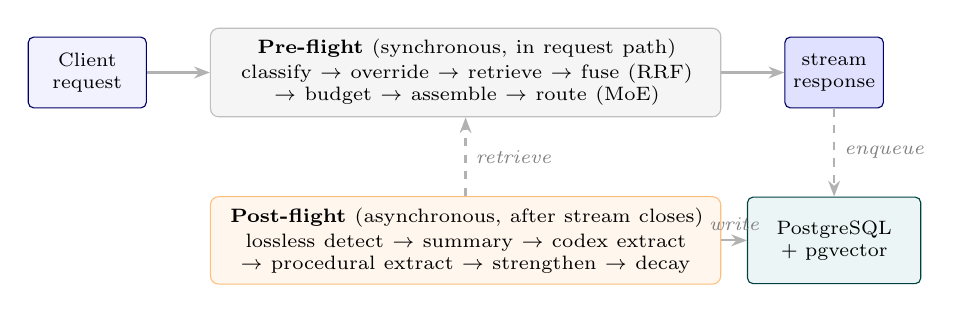
\begin{tikzpicture}[node distance=5mm]
\node[icebox, minimum width=15mm, minimum height=9mm] (client) {Client\\request};
\node[icephase, right=8mm of client, minimum height=11mm, text width=62mm] (pre)
  {Pre-flight \textnormal{(synchronous, in request path)}\\[1pt]
   \textnormal{\scriptsize classify $\to$ override $\to$ retrieve $\to$ fuse (RRF)}\\
   \textnormal{\scriptsize $\to$ budget $\to$ assemble $\to$ route (MoE)}};
\node[icebox, fill=blue!12, right=8mm of pre, minimum height=9mm] (stream) {stream\\response};
\node[icephase, fill=orange!7, draw=orange!50, below=10mm of pre, minimum height=11mm, text width=62mm] (post)
  {Post-flight \textnormal{(asynchronous, after stream closes)}\\[1pt]
   \textnormal{\scriptsize lossless detect $\to$ summary $\to$ codex extract}\\
   \textnormal{\scriptsize $\to$ procedural extract $\to$ strengthen $\to$ decay}};
\node[icestore, minimum width=22mm, minimum height=11mm] (db) at (stream |- post) {PostgreSQL\\+ pgvector};
\draw[iceflow] (client) -- (pre);
\draw[iceflow] (pre) -- (stream);
\draw[iceflowd] (stream) -- (db) node[midway, right, font=\scriptsize\itshape, gray] {enqueue};
\draw[iceflow] (post) -- (db) node[midway, above, font=\scriptsize\itshape, gray] {write};
\draw[iceflowd] (post.north) -- (pre.south) node[midway, right, font=\scriptsize\itshape, gray] {retrieve};
\end{tikzpicture}%
}
\caption{System overview. Pre-flight runs synchronously in the request path; post-flight runs asynchronously after the stream closes and feeds the next turn's retrieval.}
\label{fig:system-overview}
\end{figure}

\subsection{Request Lifecycle}

Each turn traverses a \textbf{pre-flight} phase (synchronous, in the request path) and a \textbf{post-flight} phase (asynchronous, after the stream closes).

In pre-flight, the user message is classified into topic tags, intent tags, and a single context-reliance label (Zero\_Shot, Long\_Term\_Memory, Real\_Time\_Search) by a two-stage cascade: a rule-based pre-classifier resolves obvious cases in microseconds, and on a miss a small multi-layer perceptron over a frozen \texttt{Qwen3-Embedding-0.6B} encoder resolves the rest with sub-millisecond CPU inference. Hard override rules then coerce the label---most consequentially, a conservative rule upgrading Zero\_Shot to Long\_Term\_Memory when a conversation exceeds ten turns or confidence falls below 0.95, so retrieval runs for almost every turn in a long conversation; Section~\ref{sec:limitations} discusses what that costs. A Hybrid Retrieval Orchestrator then runs the retrieval legs, fuses them with weighted Reciprocal Rank Fusion, and post-processes the fused list. A Prompt Assembler concatenates the surviving fragments with persistent memory slots, recent turns, and the live message under a stable prefix, and a Mixture-of-Experts router selects a locally-served model with per-conversation stickiness.

In post-flight, an evaluator runs lossless detection---the guiding principle in the code is that \emph{memory is earned}: a turn is stored verbatim only if dense enough, and is otherwise summarised---and dispatches idempotent extraction tasks for the knowledge graph and for procedural patterns. Scheduled workers (decay, clustering, reflection, batch summarisation, sentinel monitoring, and a weekly classifier fine-tune) maintain the stores over time; \cref{tab:workers} in the appendix lists them.

\subsection{Memory Stores}

ICE maintains four stores plus two structured overlays, all in one PostgreSQL database with the pgvector extension; every vector column is 384-dimensional because a single embedder is shared throughout.

\begin{table}[htbp]
\centering
\small
\caption{The four memory stores and the overlays. Each store is queried by one or more retrieval legs. Appendix~\ref{app:implementation} gives schemas and write paths.}
\label{tab:stores}
\begin{tabular}{@{}L{2.2cm}L{6.0cm}L{4.4cm}@{}}
\toprule
\textbf{Store} & \textbf{Purpose} & \textbf{Retrieval method} \\
\midrule
Episodic & Every conversational turn: raw text, summary, lossless flag, decay score, access count, embedding & BM25 leg; vector leg with decay weighting; session diversification \\
Codex & Temporally-versioned semantic graph: entities with aliases and properties, typed edges carrying \texttt{valid\_from}/\texttt{valid\_until}, append-only event log, snapshots & Graph traversal (BFS depth 3 over edges where \texttt{valid\_until IS NULL}); enumeration fallback \\
Procedural & Recurring behavioural patterns: trigger conditions, reinforcement count, confidence & Vector top-5 behind a hard intent gate \\
RAG & Externally-ingested documents, chunked and embedded & Vector top-5, triple-gated \\
\midrule
Memory slots & Seven server-enforced persistent slots (persona, preferences, project context, guidance, pending items, \ldots) & Prepended verbatim to every prompt \\
Context clusters & Conversation-scoped topical groupings with unit-norm centroids & Restrict episodic search to relevant clusters \\
\bottomrule
\end{tabular}
\end{table}

The \textbf{Codex} is the store most specific to conversation. Its central design lever is a three-bucket controlled relation vocabulary---\emph{property} relations overwrite, \emph{multi-valued} relations accumulate, and \emph{single-valued} relations auto-expire the prior edge of the same (source, relation) pair---with generic relations such as \texttt{is} and \texttt{has} deliberately absent so the extractor is forced to be specific. Setting \texttt{valid\_until} rather than deleting is what makes the graph temporal: an edge with \texttt{valid\_until IS NULL} is currently true, and a non-NULL value means historically superseded but still auditable. Appendix~\ref{app:codex} details the write path and entity resolution.

\textbf{Decay} is access-weighted. Three decay workers apply per-cycle multipliers of roughly 5\%, 2\%, and 1\% per day for unaccessed, accessed, and creative-tagged turns respectively, with a \emph{creative floor} clamping decay score at 0.3 for narrative turns regardless of age---long-form fiction should not be summarised away for being old. Turns below 0.1 are archived and below 0.05 moved to cold storage. Codex edges decay similarly and are demoted from active to pending below a strength threshold; procedural patterns deactivate after 180 days with fewer than three reinforcements. Crucially, decay is not one-directional: every retrieval increments a fragment's access count and restores 0.15 to its decay score, so \textbf{retrieval is a partial reversal of forgetting} and what the system used yesterday is cheaper to reach today.

\subsection{Hybrid Retrieval Orchestrator}
\label{sec:orchestrator}

The orchestrator is the core of pre-flight and the component this study measures most directly.

\textbf{Retrieval legs.} Six legs are defined: \textbf{BM25} over a Postgres tsvector of raw and summary text, filtered on decay score and archival status; \textbf{vector} with decay weighting, scoring $(1 - (\text{embedding} \Leftrightarrow \text{query}))\cdot\text{decay\_score}$, which is what distinguishes this leg from pure semantic search---a highly similar but decayed turn is down-ranked; \textbf{Codex graph traversal}; \textbf{procedural} behind a hard intent gate; \textbf{RAG}, triple-gated and global rather than conversation-scoped; and \textbf{batch summaries}, conversation-scoped. Section~\ref{sec:exercised} reports which of these actually contributed during the evaluation, and why.

\textbf{Dynamic leg weighting.} Base weights are $\{$bm25 0.8, vector 1.0, codex 0.5, procedural 0.2, rag 1.0$\}$. Five intent profiles override them---Factual\_Retrieval boosts vector and demotes codex; Generation, Ideation, and Open\_Exploration do the reverse---and two cumulative topic overrides then apply. This is the mechanism by which inferred intent conditions retrieval, and it is the least-explored lever in the system.

\textbf{Reciprocal Rank Fusion} combines the legs:
\begin{equation}
\mathrm{score}_{\mathrm{RRF}}(f) = \sum_{\ell \in \mathrm{legs}} \frac{\alpha_\ell}{k + \mathrm{rank}_\ell(f)}, \quad k = 60,
\end{equation}
where $\alpha_\ell$ is the blended leg weight and $\mathrm{rank}_\ell(f)$ starts at 1. Fragments are deduplicated \emph{during} fusion: the first occurrence is registered and later occurrences add to its score, so agreement across legs is rewarded. Because RRF consumes ranks rather than scores, heterogeneous legs need no score normalisation to be combined---which is precisely why it can rescue a lexical leg whose raw scores are on an incomparable scale (Section~\ref{sec:ablation}).

\textbf{Post-fusion curation} applies five sequential transforms, and it is these---not the number of stores---that produce ICE's fragment reduction. Additive bonuses reward keyword overlap and length and penalise very short fragments; a recency bonus favours the most recent decile but is \emph{skipped} for creative turns, because recent meta-discussion is noise for narrative work. Session diversification caps foreign conversations at three fragments each while leaving the active conversation uncapped. Deduplication hashes fragment text. A two-phase token budget then guarantees leg diversity---the best fragment of each leg is admitted first if it fits---before greedily filling the remainder. Finally the strengthening step writes back the access-count and decay-score restoration described above.

\textbf{Cluster-scoped retrieval} restricts episodic search to the most relevant topical clusters, falling back to global search when no cluster clears a threshold.

\textbf{Dynamic token budget.} A total context budget of 23{,}000 tokens less an overhead reserve leaves 21{,}200 available. A length-based recent-window fraction, reduced by token density and shifted by intent and topic, splits this between recent turns and retrieval, and a \emph{growth cap} bracketed by turn count prevents long conversations from over-allocating. Leftover budget is intentionally left unused: this is the lever that keeps the retrieved set compact and, under extreme per-turn density, averts the context overflow that sinks an unbudgeted baseline (Section~\ref{sec:stress}). On ordinary turns ICE's total token count is comparable to the baseline's---the curation shows up as fewer \emph{fragments}, not fewer tokens. A configurable subclass of the orchestrator exposes flags that switch legs and post-processing steps on and off without redefining classification or fusion; Section~\ref{sec:ablation}'s buildup uses that mechanism.

\begin{figure}[t]
\centering
\resizebox{\columnwidth}{!}{%
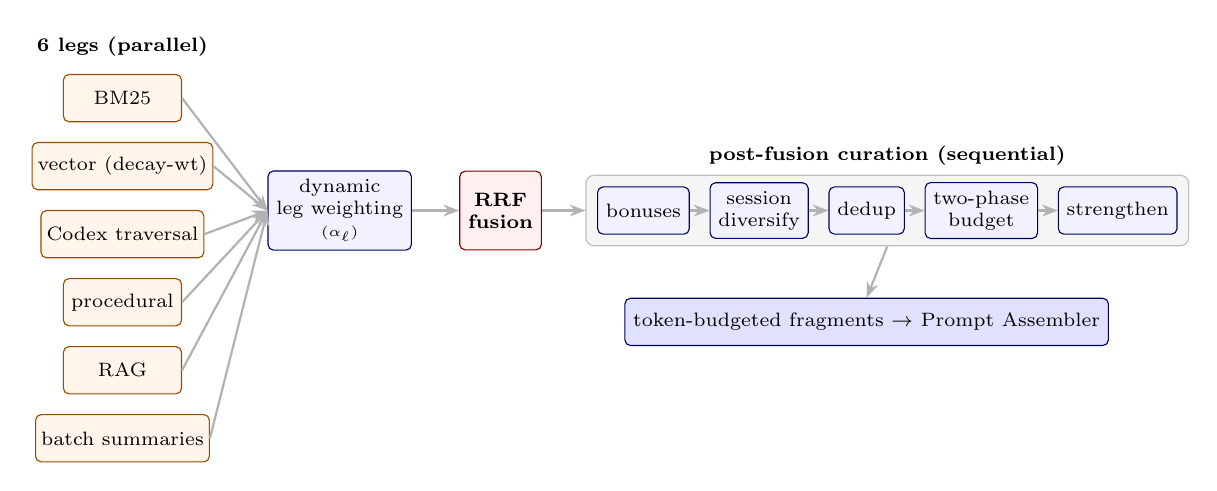
\begin{tikzpicture}[node distance=2.5mm]
\node[iceleg] (l1) {BM25};
\node[iceleg, below=of l1] (l2) {vector (decay-wt)};
\node[iceleg, below=of l2] (l3) {Codex traversal};
\node[iceleg, below=of l3] (l4) {procedural};
\node[iceleg, below=of l4] (l5) {RAG};
\node[iceleg, below=of l5] (l6) {batch summaries};
\node[font=\scriptsize\bfseries, above=1mm of l1] {6 legs (parallel)};
\node[icebox, right=8mm of l3, yshift=3mm, minimum height=10mm] (wt) {dynamic\\leg weighting\\{\tiny($\alpha_\ell$)}};
\node[icecore, right=6mm of wt, minimum height=10mm] (rrf) {RRF\\fusion};
\node[icebox, right=7mm of rrf] (t1) {bonuses};
\node[icebox, right=2.5mm of t1] (t2) {session\\diversify};
\node[icebox, right=2.5mm of t2] (t3) {dedup};
\node[icebox, right=2.5mm of t3] (t4) {two-phase\\budget};
\node[icebox, right=2.5mm of t4] (t5) {strengthen};
\begin{scope}[on background layer]
\node[icephase, fit=(t1)(t5), inner sep=4pt, label={[font=\scriptsize\bfseries]above:post-fusion curation (sequential)}] (post) {};
\end{scope}
\node[icebox, fill=blue!12, below=8mm of t3, minimum width=30mm] (out) {token-budgeted fragments $\rightarrow$ Prompt Assembler};
\foreach \l in {l1,l2,l3,l4,l5,l6} \draw[iceflow] (\l.east) -- (wt.west);
\draw[iceflow] (wt) -- (rrf);
\draw[iceflow] (rrf) -- (post);
\draw[iceflow] (t1) -- (t2); \draw[iceflow] (t2) -- (t3);
\draw[iceflow] (t3) -- (t4); \draw[iceflow] (t4) -- (t5);
\draw[iceflow] (post.south) -- (out.north);
\end{tikzpicture}%
}
\caption{Retrieval orchestrator. The legs are heterogeneous in retrieval semantics; RRF is what allows them to be combined without score normalisation; the two-phase budget guarantees leg diversity under budget pressure. Section~\ref{sec:exercised} reports which legs contributed during evaluation.}
\label{fig:orchestrator}
\end{figure}

\subsection{Prompt Assembly}

The assembler orders messages for stable-prefix reuse: a fixed system message with an inline block rendering the active memory slots; recent turns under dynamic per-turn word caps; a single user message carrying the retrieved context; a short assistant acknowledgement acting as a boundary marker so the model treats the final message as the live question rather than another history turn; and the question itself. A second budget pass at the API layer enforces a per-model word ceiling, popping procedural and episodic fragments first and preserving document and graph fragments because they are hardest to recompute. Appendix~\ref{app:assembly} gives the full ordering and caps.

This assembler is part of what the evaluation compares. The baseline receives retrieved chunks and the question; ICE receives fused, curated fragments \emph{plus} slots, a recent window, and structural boundaries. That is a deliberate full-system-versus-standard-RAG comparison, stated explicitly in Section~\ref{sec:exp2-env} so it is not mistaken for an accident.

%======================================================================
\section{Evaluation Protocol}
\label{sec:exp-design}

\subsection{Why a New Protocol Was Needed}

Our first evaluation attempt measured retrieval \emph{precision}: did the orchestrator retrieve the fragment whose timestamp the ground-truth file named? It failed for two compounding reasons. The first we call the \emph{stateless pronoun problem}: probes were extracted from their conversations and tested in a vacuum, so a question like ``you mentioned the current script saves nothing'' reached the orchestrator stripped of every surrounding turn, and the system returned fragments that were mathematically correct in isolation and functionally useless. The second was an \emph{incompetent judge}: a 7B grading model scored 0 for fragments a human immediately recognised as the exact session being asked about. Manual re-scoring of a subset produced 31\% precision against the automated 13.87\%, and the gap was the judge, not the retrieval.

Two conclusions followed, and they define LSREP. Evaluating retrieval intermediates is the wrong level of abstraction---a fragment that is irrelevant at turn 100 may be critical at turn 800, and a fragment differing from the reference may be equally valid---so the system must answer real questions and the \emph{answers} must be judged. And if memory accumulation is the object of study, the same questions must be asked at multiple points in time, not once at the end.

\subsection{LSREP}
\label{sec:lsrep}

LSREP freezes a historical conversation at a temporal slice $T_n$, reconstructs the entire database and memory-lifecycle state exactly as it existed at that moment, injects evaluation probes, and evaluates the answers with an independent judge.

The general procedure: for each conversation, determine the turn count $L$ and select checkpoints; wipe the target database and inject turns $T_1 \ldots T_{n-1}$ sequentially into episodic memory, preserving relative or real timestamps; trigger the background workers synchronously, so decay computes initial scores, the graph extractor builds entities and edges, the procedural extractor scans for behavioural motifs, and the clustering worker aggregates related turns; then administer the probes and judge the answers. The protocol is system-agnostic: it requires only that the system under test expose a chat endpoint and that its persistent state be reconstructible from a turn sequence.

We ran two instantiations. \textbf{Experiment~1 is a pilot} whose role was to expose measurement flaws and immature subsystems; it is reported in Appendix~\ref{app:exp1}, which also tabulates the two instantiations side by side (\cref{tab:exp-diff}), and it is referenced here only where it explains a design change. \textbf{Experiment~2 is the substantive evaluation}, and \textbf{Experiment~3} is a cumulative ablation explaining why the mature system behaves as it does.

\subsection{The Standing of a Purpose-Built Protocol}
\label{sec:lsrep-standing}

A protocol introduced in the same paper as the system it measures invites an obvious objection: that the instrument was fitted to the result. The objection is the right one to raise, and we would rather answer it than let it stand implicitly. Four things bear on it, and we state the falsifier for each.

\textbf{The protocol was built from a failure, not a success.} LSREP's design is a direct response to Experiment~1, a pilot in which the system scored \emph{worse} than its own baseline on every metric---4.04 against 4.06 on score, 47\% more tokens, higher hallucination---and in which a token-accounting error invalidated the efficiency claim once corrected (Appendix~\ref{app:exp1}). The two defining decisions of the protocol, judging answers rather than retrieval intermediates and asking the same question at many points in time, were forced by that failure. An instrument designed to flatter would not have been derived from a result this unflattering, and would not report the pilot at all.

\textbf{It returns unflattering results on the mature system too.} Under LSREP, ICE \emph{ties} the baseline on answer quality (paired $\Delta = +0.00$, CI $[-0.07, +0.07]$), one of its design levers regresses (the dynamic budget's step is $-0.11$), and the ablation's headline is that the system's own lexical leg is actively harmful until fusion corrects it. A metric fitted to a system does not report a tie as its central quality finding. \emph{Falsifier:} if the protocol's scoring rewarded structures only ICE produces, the baseline could not have tied it.

\textbf{It is specified independently of the system.} Admissibility requires two things---a chat endpoint, and persistent state reconstructible from a turn sequence---neither of which is ICE-specific. The vector-RAG baseline runs under the identical protocol, with the same judge, the same probes, the same checkpoints and the same evolving ground truth; the conditions differ only in the system behind the endpoint. \emph{Falsifier:} if any ICE component were required for the protocol to execute, or if the scoring rubric named an ICE-internal structure, the independence claim would fail. Neither is the case, and the released harness is the check.

\textbf{The protocol is separable from our corpus.} This matters most, because the corpus is the part we cannot share. LSREP ingests ordinary chat-log exports, which most platforms provide, so a reader can run the protocol on their own history at whatever length they have accumulated. What we are asking to be taken on trust is therefore narrower than it first appears: not our numbers, but the claim that the procedure is well defined---and that claim is checkable against the code without our data.

None of this makes a purpose-built protocol a substitute for standard benchmarks, and we do not present it as one. The two answer different questions, as Section~\ref{sec:related-eval} sets out, and a memory system should be able to face both: an established benchmark tests the regime the field already measures, while LSREP measures a regime it does not. This study adds the complete evidence-only LongMemEval oracle as a public diagnostic, but not the distractor-heavy LongMemEval-S evaluation; Section~\ref{sec:lme-oracle} reports why that progression stopped. The result is therefore a limitation on ICE's transfer, not a claim that LSREP replaces external validation.

\subsection{Experiment 2 Environment}
\label{sec:exp2-env}

\textbf{System under test.} Experiment 2 evaluated the mature system: the classifier backbone upgraded to Qwen3-Embedding-0.6B with the head retrained from scratch; a trained micro-NER model replacing the pilot's regex entity tagger, so the graph extractor grounds on real entity detection ($\sim$95\% recall); the conservative routing override added; the static budget and uncapped sliding window replaced by the unified dynamic token budget of Section~\ref{sec:orchestrator}; and cluster-scoped retrieval introduced.

\textbf{Protocol instantiation.} Rather than many conversations at isolated checkpoints, Experiment 2 follows four long-horizon conversations across their entire lifespan. Three choices differ sharply from the pilot. \emph{(1)~Continuous replay with preserved state}: each conversation is replayed chronologically into one fresh deployment, and memory stored at an early checkpoint remains available at every later one; a simulated memory lifecycle---decay, edge decay, procedural decay, reflection, clustering, consolidation, sentinel monitoring---runs \emph{between} checkpoints, so retrieval reflects aged, consolidated memory rather than fresh storage. \emph{(2)~Automatic, leg-aware probe generation}: probes are generated at each checkpoint from a sampled history window (first 5 turns, last 10 before the checkpoint, 15 random from between) using only information available up to that checkpoint, explicitly targeting specific legs, and each requires a unique temporal anchor to prevent ambiguity across hundreds of turns. These are combined with 72 hand-written probes inherited from the pilot. \emph{(3)~Incremental evaluation}: every probe whose origin is at or before a checkpoint is re-evaluated at that checkpoint, so a probe generated early is scored repeatedly as history accumulates---which is what makes longitudinal memory growth directly observable.

\textbf{Evolving ground truth.} The pilot's single frozen reference is replaced by a three-stage temporal-refinement pipeline: \emph{forensic regeneration} of the origin-checkpoint answer under a stricter, evidence-oriented prompt that records temporal provenance; \emph{temporal anchoring}, attaching to each probe an anchor identifying the fact or event it tracks; and \emph{forward propagation}, updating each answer at every later checkpoint when new content contradicts, updates, or extends it, with anchor-preservation checks guarding against silent drift to a superficially similar later event. Each probe therefore carries a temporally evolving reference document rather than a static answer---necessary because otherwise a system that correctly \emph{updated} a fact would score worse than one repeating an outdated one.

\textbf{Scoring.} Experiment 2 adds temporal-aware scoring (an answer loses points for reporting a superseded fact even if it was once correct) and inference credit (a specific, evidence-consistent detail not explicitly in the reference is rewarded rather than flagged as fabrication).

\textbf{Human verification, not score alteration.} Two pieces of human involvement need stating precisely, because ``manually verified'' can be misread as ``scores were adjusted by hand.'' They were not; the human role was verification and correction of the judge's own labels, not substitution of human judgement for the judge's. First, the 72 hand-written probes inherited from the pilot were re-evaluated by hand against both their absolute scores and their tournament rankings, so a human-authored, human-checked slice sits inside the benchmark alongside the automatically generated and automatically judged probes---not merely the model's own self-consistency. Second, every hallucination flag across all 1{,}211 probes was manually audited. This was necessary because the automated judge was systematically too harsh across \emph{all four} conditions---generalist and MoE, ICE and vector alike---whenever an answer contained a specific, true, directly relevant detail that was simply absent from the necessarily condensed ground-truth dossier; the judge tended to flag such details as unsupported rather than recognise them as correct supplementary information. The audit corrected these false positives wherever a detail was verifiably true against the source conversation, applying the same standard to every condition; it did not remove flags for genuine fabrications, and we deliberately did not over-correct by crediting speculative or unverifiable additions. This audit covers Experiment 2 only; Experiment 3 uses the automated judge's hallucination labels unmodified, for the bias reasons in Section~\ref{sec:limitations}.

\textbf{Judge.} Scoring free-form answers with a language model follows now-standard practice~\citep{zheng2023judging,liu2023geval}, and inherits its known failure modes: judges are sensitive to answer position and verbosity and are not fair evaluators by default~\citep{wang2024unfair}. We mitigate rather than assume this away---blind pairwise comparison for win rate, a fixed rubric at temperature 0.0, a judge model disjoint from every answering model, and the hand-audited slice described above; Section~\ref{sec:limitations} states what remains uncontrolled. Both experiments use the same independent judge, \texttt{gemma-4-12B-AWQ} served on SGLang with a 150{,}000-token context at temperature 0.0 and deterministic decoding, never used for retrieval, generation, probe generation, or ground-truth construction. The extraction rules---strict neutrality, verbatim anchor preservation, temporal dominance, third-person attribution---are shared; Experiment 2 applies them through the evolving-dossier pipeline rather than a single pass.

\textbf{Conditions.} A four-condition matrix: \textbf{Vector RAG (generalist)}---single-leg pgvector similarity, top-30, no decay weighting, classification, or fusion, on a generalist model; \textbf{Vector RAG (MoE)}---same retrieval, expert-routed; \textbf{Full ICE (generalist)}---all legs enabled, RRF fusion, classification, decay weighting, dynamic budget, post-fusion curation; and \textbf{Full ICE (MoE)}. Both use the same embedder and database. The baseline is a standard single-leg vector-RAG---top-30 similar turns assembled with the question---while the ICE conditions run the full system, fused retrieval \emph{plus} ICE's prompt assembler. The comparison is therefore \emph{full memory system versus standard vector-RAG}, which is what a deployment decision actually looks like: ICE's curation deliberately governs what context is assembled, not merely which fragments are retrieved.

\textbf{A note on replay.} Because history is \emph{replayed} rather than lived, the reinforcement that normally strengthens frequently referenced memories during use is largely absent---the primary reinforcement signal becomes the evaluation probes themselves. A concept referenced dozens of times in real use and one mentioned once therefore look more alike under replay than they would in deployment. This changes the state trajectory, but its direction is not guaranteed: reinforcement can promote useful evidence or amplify an early retrieval error. Experiment~2 should therefore be read as performance under the specified replay process, not as a lower or upper bound on deployment.

\subsection{Metrics}


No single metric captures memory quality, which is why we report several and read them together. Absolute \emph{score} conceals the cost at which quality was achieved; \emph{SPF} and \emph{TUR} expose that cost, which is the axis on which a curated memory system must distinguish itself from a firehose. \emph{Win rate} is the noise-robust relative signal, sidestepping the absolute-scale drift that makes raw 1--5 judgements hard to compare across hundreds of probes, and it often separates systems that tie on mean score. \emph{Hallucination} and \emph{fragment count} guard the two ways a system can look good on score and fail in practice---fabrication, and context bloat. \emph{Recency delta} is the longitudinal signal unique to this setting: whether answers \emph{improve} as memory accumulates, which a static-corpus baseline structurally cannot exhibit.

Where confidence intervals are reported they are 95\% percentile-bootstrap intervals over 10{,}000 resamples of probes with replacement, computed on the same per-probe records that produce the point estimates and including the published missing-score imputation; paired score differences are computed within-probe before resampling. The scripts that produce them are released with the harness.

%======================================================================
\section{Results}
\label{sec:results}

The pilot (Experiment~1) is reported in Appendix~\ref{app:exp1}. Its short version: honestly measured, the immature system was \emph{worse} than the vector baseline on every metric---4.04 against 4.06 on score, 47\% more tokens, higher hallucination---and a token-accounting audit found the reported context size had omitted the recent-turn sliding window, which invalidated any efficiency claim once corrected. That result drove the mature design and is the reason this paper reports the pilot as diagnostic rather than as evidence.

\subsection{Mature System Evaluation}
\label{sec:exp2}

\cref{tab:exp2-global} reports the four conditions on the three-conversation view (Dataset C excluded; 1{,}057 probes). Per-conversation, score-distribution, and temporal-quality breakdowns are in Appendix~\ref{app:exp2-detail}.

\begin{table}[htbp]
\centering
\small
\caption{Experiment 2, global comparison, Dataset C excluded (1{,}057 probes across 3 conversations). On the conversations where both systems can generate usable answers, ICE ties the vector baseline on mean score, injects 32\% fewer fragments, and wins 30.6\% of head-to-head comparisons against 21.2\%.}
\label{tab:exp2-global}
\resizebox{\textwidth}{!}{%
\begin{tabular}{@{}lccccccc@{}}
\toprule
\textbf{Condition} & \textbf{Score} & \textbf{Tokens} & \textbf{Frags} & \textbf{SPF} & \textbf{TUR} & \textbf{Win \%} & \textbf{Hall. \%} \\
\midrule
Vector RAG generalist & 4.25 $\pm$ 1.09 & 21{,}025 & 30.0 & 0.14 & 0.20 & 21.2 & 20.5 \\
Vector RAG MoE        & 4.24 $\pm$ 1.04 & 21{,}025 & 30.0 & 0.14 & 0.20 & 19.2 & 17.4 \\
Full ICE generalist   & 4.26 $\pm$ 1.08 & 22{,}411 & 20.4 & 0.21 & 0.19 & \textbf{30.6} & 19.6 \\
Full ICE MoE          & \textbf{4.28} $\pm$ 0.99 & 22{,}411 & 20.4 & 0.21 & 0.19 & 29.0 & 19.9 \\
\bottomrule
\end{tabular}%
}
\end{table}

The mean-score difference between ICE generalist and vector generalist is $+0.01$ (4.26 vs.\ 4.25). A paired per-probe bootstrap---both conditions answer the same probes, so the difference is taken within-probe before resampling---places it at $+0.00$ with a 95\% CI of $[-0.07, +0.07]$: a tightly estimated statistical tie rather than an ambiguous one. The secondary metrics carry the interesting content.

\textbf{Efficiency.} ICE injects 32.0\% fewer fragments (20.4 vs.\ 30.0) at the same quality, giving an SPF of 0.21 against 0.14---a 50\% improvement in quality per fragment. It uses 6.6\% \emph{more} tokens (22{,}411 vs.\ 21{,}025). That overage is not fragment bloat: it is prompt structure the baseline never receives. Every ICE prompt carries a fixed instruction preamble, a persistent-context header, a retrieved-context header and a boundary acknowledgment turn---about 195 tokens of static scaffolding---plus any active memory slots verbatim and a window of recent conversation turns, while the baseline is served only its retrieved fragments and the question. The comparison is therefore full-system-versus-standard-RAG rather than fragment-versus-fragment, and the accounting is deliberately unflattering to us: ICE spends its extra tokens on structure and recency while retrieving a third fewer fragments. We state it plainly because it is the opposite of the claim such systems usually make: the win is in \emph{how many things} the model must reconcile, not in raw token count. Whether that scaffolding earns its cost is \emph{untested}. We never ran ICE's retrieval behind the baseline's bare prompt, so we cannot say whether stripping the preamble and the recent-turns window would have been cheaper at equal quality, cheaper at worse quality, or neither: the tokens and the answer quality move together in our design and we did not separate them. This is a controlled comparison the study omits, not a result it reports, and it is the first arm we add in the follow-up.

\textbf{Preference.} The head-to-head win rate is the cleanest signal and it is statistically robust: ICE generalist wins 30.6\% of tournament appearances (95\% CI $[27.9, 33.4]$) against the baseline's 21.2\% ($[18.8, 23.7]$), and the intervals do not overlap. When the two systems disagree, ICE is more often preferred. Hallucination rates are close (19.6\% vs.\ 20.5\%).

\textbf{Fragment--score correlation} shows a qualitative difference rather than a quantitative one. ICE generalist has $r = +0.193$ (MoE $+0.246$); vector generalist has $r = -0.015$ (MoE $-0.030$). For ICE, retrieving more fragments goes with better answers; for the baseline, retrieving more goes with worse. Same metric, opposite sign---a system whose retrieved fragments correlate negatively with answer quality is, in a deep sense, a system that does not know what it is doing.

\textbf{Longitudinal behaviour.} \cref{fig:longitudinal} plots mean probe score against turn-index bin. All four conditions track closely through early and middle bins---the tie is visible as four overlapping curves. The separation appears at the deepest bin (turn 1{,}100 of Dataset B): both vector conditions drop sharply, to 3.80 and 3.87, while both ICE conditions hold at 4.18 and 4.14. The baseline's retrieval cannot reach across 1{,}000+ turns of history, and the gap opens precisely where that reach matters.

\textbf{Token efficiency is not a constant, and the pooled average hides a crossover.} The 6.6\% figure above is an average over conditions that differ sharply, and two mechanisms push against each other. Per-turn \emph{density} favours ICE: the baseline retrieves a fixed top-30, so its injected tokens scale with how large each turn is, without bound. Conversation \emph{length} favours the baseline: ICE's growth cap deliberately widens the budget as turns accumulate ($2{,}000 + 150n$ below 30 turns, then $5{,}000 + 100(n-30)$, then $10{,}000 + 30(n-100)$), while top-30 is indifferent to how long a conversation has run. \cref{tab:token-crossover} contrasts the first and last quartile of each conversation, paired per probe and bootstrapped. Within every conversation the baseline is effectively flat and only ICE moves, so the trend is a property of the budget rather than of which conversation is being read.

The clearest case is Dataset D, where the effect reverses sign inside a single conversation: ICE injects 2{,}309 fewer tokens than the baseline over the first quartile and 4{,}994 \emph{more} over the last, both intervals excluding zero, against a baseline that barely moves. Dataset A shows the same erosion without a reversal, and Dataset C shows density overwhelming the effect entirely---there the baseline sits near 87{,}000 tokens and ICE is cheaper on every probe at every position. The practical reading is that a per-query budget buys the most when turns are dense and least when a conversation is long and sparse. What it does \emph{not} show is that the extra spend is wasted. Paired per-probe score differences move the other way: from the first quartile to the last they improve in all four conversations---$+0.19$ to $+0.20$ on Dataset A, $-0.23$ to $+0.18$ on B, $+3.18$ to $+3.42$ on C, and $-0.07$ to $+0.16$ on D---so the conversations where ICE's relative cost rises are also the ones where its relative quality rises, consistent with the long-horizon divergence in \cref{fig:longitudinal}. We resist the causal reading: the budget was never varied independently of the retrieval it funds, so these are correlated consequences of accumulated memory, not a measured return on tokens. What it does license is narrower---a cap keyed to \emph{turn count} spends on a schedule rather than on evidence. Replacing fill-to-cap with a marginal-relevance stopping rule would let the same budget be justified per query rather than per position, and it is the same fix the ablation's dynamic-budget regression pointed at.

\begin{table}[htbp]
\centering
\small
\caption{Token cost by position within each conversation: first quartile of probes versus last. $\Delta$ is the paired per-probe difference (ICE minus baseline; negative means ICE is cheaper) with a 95\% bootstrap interval, and ``cheaper'' is the share of probes on which ICE injected fewer tokens. The baseline is close to flat within each conversation; ICE's cost rises with position in all four.}
\label{tab:token-crossover}
\begin{tabular}{@{}llrrr@{}}
\toprule
\textbf{Dataset} & \textbf{Position} & \textbf{Paired $\Delta$} & \textbf{95\% CI} & \textbf{ICE cheaper} \\
\midrule
\multirow{2}{*}{A (Creative, 290 turns)} & first quartile & $-8{,}034$ & $[-8{,}650, -7{,}451]$ & 100\% \\
                                          & last quartile  & $-2{,}284$ & $[-2{,}766, -1{,}800]$ & 91\% \\
\midrule
\multirow{2}{*}{B (Long-form, 1{,}119 turns)} & first quartile & $+3{,}766$ & $[+3{,}133, +4{,}394]$ & 18\% \\
                                               & last quartile  & $+1{,}288$ & $[+476, +2{,}075]$ & 35\% \\
\midrule
\multirow{2}{*}{C (Technical, 325 turns)} & first quartile & $-70{,}731$ & $[-79{,}067, -63{,}734]$ & 100\% \\
                                           & last quartile  & $-68{,}854$ & $[-88{,}105, -53{,}696]$ & 100\% \\
\midrule
\multirow{2}{*}{D (Academic, 251 turns)} & first quartile & $-2{,}309$ & $[-3{,}112, -1{,}521]$ & 69\% \\
                                          & last quartile  & $+4{,}994$ & $[+4{,}362, +5{,}609]$ & 5\% \\
\bottomrule
\end{tabular}
\end{table}

\begin{figure}[t]
\centering
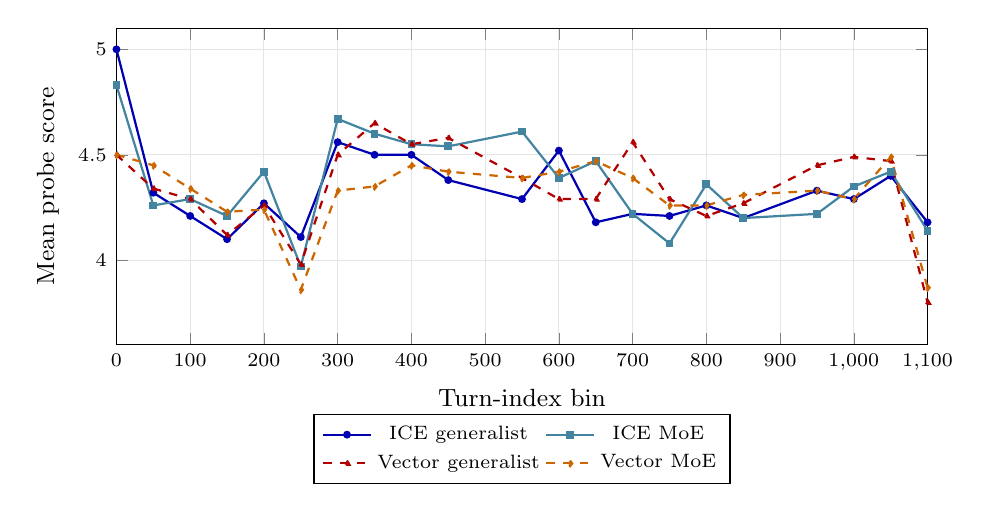
\begin{tikzpicture}
\begin{axis}[
    width=0.98\columnwidth, height=5.6cm,
    xlabel={\small Turn-index bin}, ylabel={\small Mean probe score},
    ylabel near ticks,
    xmin=0, xmax=1100, ymin=3.6, ymax=5.1,
    tick label style={font=\scriptsize},
    legend style={font=\scriptsize, at={(0.5,-0.22)}, anchor=north, legend columns=2},
    grid=major, grid style={gray!20},
]
\addplot[blue!70!black, thick, mark=*, mark size=1pt] coordinates
 {(0,5) (50,4.32) (100,4.21) (150,4.1) (200,4.27) (250,4.11) (300,4.56) (350,4.5) (400,4.5) (450,4.38) (550,4.29) (600,4.52) (650,4.18) (700,4.22) (750,4.21) (800,4.26) (850,4.2) (950,4.33) (1000,4.29) (1050,4.4) (1100,4.18)};
\addplot[cyan!60!black, thick, mark=square*, mark size=1pt] coordinates
 {(0,4.83) (50,4.26) (100,4.29) (150,4.21) (200,4.42) (250,3.97) (300,4.67) (350,4.6) (400,4.55) (450,4.54) (550,4.61) (600,4.39) (650,4.47) (700,4.22) (750,4.08) (800,4.36) (850,4.2) (950,4.22) (1000,4.35) (1050,4.42) (1100,4.14)};
\addplot[red!70!black, thick, dashed, mark=triangle*, mark size=1pt] coordinates
 {(0,4.5) (50,4.34) (100,4.29) (150,4.12) (200,4.26) (250,3.98) (300,4.5) (350,4.65) (400,4.55) (450,4.58) (550,4.39) (600,4.29) (650,4.29) (700,4.56) (750,4.29) (800,4.21) (850,4.27) (950,4.45) (1000,4.49) (1050,4.47) (1100,3.8)};
\addplot[orange!80!black, thick, dashed, mark=diamond*, mark size=1pt] coordinates
 {(0,4.5) (50,4.45) (100,4.34) (150,4.23) (200,4.24) (250,3.86) (300,4.33) (350,4.35) (400,4.45) (450,4.42) (550,4.39) (600,4.42) (650,4.47) (700,4.39) (750,4.26) (800,4.26) (850,4.31) (950,4.33) (1000,4.29) (1050,4.49) (1100,3.87)};
\legend{ICE generalist, ICE MoE, Vector generalist, Vector MoE}
\end{axis}
\end{tikzpicture}
\caption{Longitudinal mean score by turn-index bin (1{,}057 probes, Dataset C excluded; real per-bin data). The four conditions track closely mid-conversation, but at the final turn-1{,}100 bin---the deep long-horizon regime of Dataset B---both vector conditions drop sharply while both ICE conditions hold.}
\label{fig:longitudinal}
\end{figure}

\textbf{Routing.} The global MoE-versus-generalist score delta is $+0.01$ for ICE and $-0.02$ for vector; the effect is too small to claim in either direction. MoE gives a 3.1\% hallucination reduction under vector and a 0.3\% increase under ICE, and no token savings. The router ran on every probe and moved nothing---a genuine null, and we return to its significance in Section~\ref{sec:exercised}.

\textbf{Memory maturity and reliability.} Simulated decay days at the final checkpoint were 93 for Dataset B, 24 for A, 27 for C, 20 for D. Gating failures---probes where the classifier blocked retrieval that was needed---fell from 22 in the pilot to 2 here, the single largest reliability improvement in the mature deployment.

\textbf{Human-verified slice.} The 72 hand-written probes were scored entirely by hand, both an absolute 1--5 score and a blind, anonymised tournament ranking, giving a human-authored, human-judged slice inside the benchmark (\cref{tab:manual}). Here the picture is far less equivocal than the automated tie: both ICE conditions score around 4.3 against the baselines' 3.1, and the paired ICE-minus-baseline difference is $+1.21$ (95\% CI $[+0.81, +1.61]$), decisively excluding zero. Two readings are consistent with this and we lean on neither. The optimistic one: the automated judge---shown in Section~\ref{sec:limitations} to be systematically harsh---\emph{understates} ICE's advantage, so the headline tie is a conservative lower bound. The cautious one: these 72 are the harder, more memory-dependent, author-written questions on which stored context matters most, and a single scorer, even blinded per probe, cannot be assumed unbiased. The slice's dependable value is narrower but real: it is an independent check that the automated tie is not concealing an ICE \emph{deficit}. The within-ICE tournament asymmetry---the MoE variant taking 69.4\% of first places despite a marginally lower mean---is not stable at this sample size and should not be read as an MoE effect.

\begin{table}[htbp]
\centering
\small
\caption{Human-verified slice (72 hand-scored probes, independent of the automated judge). Paired ICE-versus-vector is $+1.21$ (95\% CI $[+0.81, +1.61]$), in contrast to the automated tie over all 1{,}057 probes---consistent with the automated judge being conservative. Single scorer; blind per-probe tournament ranking.}
\label{tab:manual}
\begin{tabular}{@{}lccc@{}}
\toprule
\textbf{Condition} & \textbf{Score} & \textbf{95\% CI} & \textbf{Win \%} \\
\midrule
Vector RAG (generalist) & 3.10 & $[2.75, 3.44]$ & 5.6 \\
Vector RAG (MoE)        & 3.22 & $[2.88, 3.54]$ & 8.3 \\
Full ICE (generalist)   & 4.31 & $[4.11, 4.49]$ & 16.7 \\
Full ICE (MoE)          & 4.24 & $[4.01, 4.43]$ & \textbf{69.4} \\
\bottomrule
\end{tabular}
\end{table}

\subsection{Stress Test: Context Overflow Under Extreme Density}
\label{sec:stress}

Dataset C contains architecture documents that frequently exceed 8{,}000 tokens in a single turn. The vector baseline, which always retrieves the top-30 fragments with no per-query budget, injects a mean of 88{,}061 tokens---failed cases reach 100{,}505---overwhelming the model's context window. Of 154 probes, 145 fail with a score of 1, a 94.2\% failure rate. The retrieval subsystem did find relevant information; the generation model could not process the assembled context and produced empty or degenerate responses. ICE, with its dynamic budget capping retrieval, holds a mean of 19{,}953 tokens and a mean score of 4.33.

\begin{table}[htbp]
\centering
\small
\caption{Stress test on Dataset C (154 probes). The vector baseline collapses because it has no token-budget cap. ICE survives with a mean score of 4.33 and 77\% fewer tokens injected. The baseline's 0\% hallucination rate is an artefact: 94.2\% of its responses are complete failures, so there is no answer to evaluate.}
\label{tab:stress}
\resizebox{\textwidth}{!}{%
\begin{tabular}{@{}lrrrrrrrr@{}}
\toprule
\textbf{Condition} & \textbf{Score} & \textbf{Tok.} & \textbf{Frags} & \textbf{SPF} & \textbf{TUR} & \textbf{Hall \%} & \textbf{Win \%} & \textbf{Overflow \%} \\
\midrule
Vector RAG generalist & 1.23 & 88{,}061 & 30 & 0.04 & 0.01 & 0.0* & 1.9 & \textbf{94.2} \\
Vector RAG MoE        & 1.10 & 88{,}061 & 30 & 0.04 & 0.01 & 0.0* & 4.5 & 97.4 \\
Full ICE generalist   & \textbf{4.33} & 19{,}953 & 10 & \textbf{0.43} & \textbf{0.22} & 41.4 & 43.5 & 3.9 \\
Full ICE MoE          & 4.03 & 19{,}953 & 10 & 0.40 & 0.20 & 40.8 & \textbf{50.0} & 16.2 \\
\bottomrule
\end{tabular}%
}
\end{table}

The score distributions are far apart. ICE generalist: 3.9\% at score 1, 5.2\% at 2, 11.7\% at 3, 12.3\% at 4, 66.9\% at 5. The baseline: 94.2\% at score 1, nothing at 2--4, 5.8\% at 5. ICE's SPF of 0.43 is more than ten times the baseline's 0.04.

The 41.4\% hallucination rate for ICE here deserves a careful note, because read naively it looks like a defect. ICE is attempting a difficult question and sometimes gets it wrong. The baseline is not attempting at all, so it never hallucinates; a 0\% rate here is not evidence of reliability but evidence of absence. The rate reflects task difficulty on a dataset where the system has far more material to work with, not a failure mode unique to ICE.

\textbf{Information density as a benchmark dimension.} Turn count alone is an insufficient measure of difficulty. Dataset B is the greatest challenge in \emph{temporal horizon}; Dataset C is a different challenge entirely, \emph{extreme information density}. The benchmark surfaced two distinct stress dimensions, and the second was not designed---it emerged when the first few probes returned errors.

\textbf{What the headline numbers look like with Dataset C included.} \cref{tab:exp2-global} deliberately excludes Dataset C, so the reported tie reflects conditions under which both systems can produce an answer; a 94.2\% failure rate would otherwise dominate any aggregate without saying anything about answer \emph{quality}. So that this choice is not mistaken for cherry-picking, \cref{tab:exp2-alldata} reports the same four conditions over \emph{all} 1{,}211 probes.

\begin{table}[htbp]
\centering
\small
\caption{Experiment 2 over all four conversations, Dataset C included (1{,}211 probes). Including the conversation where the baseline collapses does not merely narrow the gap---it \emph{reverses} it: the baseline falls to 3.87 while ICE rises slightly to 4.27. The win-rate and efficiency gaps both widen relative to \cref{tab:exp2-global}.}
\label{tab:exp2-alldata}
\begin{tabular}{@{}lrrrrrr@{}}
\toprule
\textbf{Condition} & \textbf{Score} & \textbf{Tokens} & \textbf{Frags} & \textbf{SPF} & \textbf{Win \%} & \textbf{Hall.\ \%} \\
\midrule
Vector RAG generalist & 3.87 $\pm$ 1.47 & 29{,}550 & 30.0 & 0.13 & 18.7 & 20.2 \\
Vector RAG MoE        & 3.84 $\pm$ 1.45 & 29{,}550 & 30.0 & 0.13 & 17.3 & 15.7 \\
Full ICE generalist   & \textbf{4.27} $\pm$ 1.09 & 22{,}099 & 19.1 & \textbf{0.22} & \textbf{32.3} & 22.3 \\
Full ICE MoE          & 4.25 $\pm$ 1.03 & 22{,}099 & 19.1 & 0.22 & 31.7 & 22.5 \\
\bottomrule
\end{tabular}
\end{table}

On this all-data view the paired per-probe difference is $+0.40$ (95\% CI $[+0.31, +0.49]$), decisively excluding zero; on the stress test alone it is $+3.10$ ($[+2.85, +3.33]$). This is a stronger result than the headline tie suggests, and we want to be explicit about why we did not lead with it. Excluding Dataset C from the primary comparison is the more conservative choice, not the more flattering one: it isolates ``does ICE cost anything when both systems can answer'' from ``does ICE survive when the baseline cannot,'' so a reader can evaluate each claim on its own evidence rather than one number smuggling in the other. Reporting only the all-data table would invite the fair objection that a single catastrophic-failure conversation does all the work of the headline; reporting only the excluded-C table would omit a real finding. \cref{tab:stress} exists so the stress result is visible and auditable on its own, and \cref{tab:exp2-alldata} exists so a reader can see exactly how much the exclusion was doing. We consider both necessary and neither sufficient alone.

\subsection{Feature Ablation}
\label{sec:ablation}

To understand which mechanisms matter, we ran a cumulative feature buildup on Dataset B (67 probes, fully mature memory state, single pass), constructing the system incrementally from a bare-vector baseline with each step adding exactly one feature and preserving all previous ones. The answering model here is Qwen3-14B-AWQ rather than Experiment 2's 26B generalist; the independent Gemma-4 12B judge is unchanged. Absolute scores are therefore not comparable across experiments, and relative within-probe deltas are the object of interest. \cref{tab:ablation-main} gives the CI-robust steps; the full fifteen-row table, the recency breakdown, and the waterfall chart are in Appendix~\ref{app:ablation}.

\begin{table}[htbp]
\centering
\small
\caption{The ablation steps that clear a paired within-probe bootstrap 95\% CI (10{,}000 resamples, 67 probes scored under every condition), with the endpoints for context. Every other step's interval spans zero; the full table is \cref{tab:ablation-full}. The single-leg vector baseline is a reference point, not a buildup step.}
\label{tab:ablation-main}
\begin{tabular}{@{}lrrl@{}}
\toprule
\textbf{Step} & \textbf{Score} & \textbf{Paired $\Delta$} & \textbf{95\% CI} \\
\midrule
bare\_vector             & 3.27 & ---     & --- \\
$+$BM25                  & 2.52 & $-0.74$ & $[-1.14, -0.36]$ \quad excludes 0 \\
$+$RRF                   & 3.36 & $+0.82$ & $[+0.39, +1.24]$ \quad excludes 0 \\
\multicolumn{4}{@{}l@{}}{\emph{\quad nine further steps, all spanning zero (Appendix~\ref{app:ablation})}} \\
full\_ice                & 3.38 & $-0.03$ & $[-0.29, +0.23]$ \\
\midrule
vector\_baseline (ref.)  & 3.42 & ---     & --- \\
\bottomrule
\end{tabular}
\end{table}

\textbf{Adding an unfused lexical leg is harmful} ($-0.74$, $[-1.14,-0.36]$). Unfused lexical matches flood the context and actively hurt answer quality---naive multi-leg retrieval is worse than single-leg retrieval, which is the opposite of the intuition that motivates most multi-signal designs.

\textbf{Rank fusion is corrective} ($+0.82$, $[+0.39,+1.24]$). Adding RRF on top recovers the damage. Its role is precisely that: recovery. Neither RRF-on-vector nor the fully built configuration is statistically distinguishable from the single-leg baseline on answer quality---both contrasts span zero, consistent with the Experiment 2 tie. RRF is the mechanism that makes multi-signal retrieval \emph{safe}, not a lever that lifts quality above a strong baseline. We state this deliberately because the earlier draft of this work claimed RRF was the single most impactful component; the paired intervals do not support that, and the corrected claim is the smaller one.

The remaining steps must be read with care, and Section~\ref{sec:exercised} explains why: several toggled features were not functioning or not varying at the snapshot, so their near-zero deltas measure nothing about the mechanism. The genuinely \emph{measured} neutrals---features that ran and moved nothing---are cluster restriction and session diversification ($\Delta \leq 0.01$). One design lever is implicated negatively: the dynamic budget's step is $-0.11$, because its fill-to-cap policy allocates more tokens to longer conversations and over-injects on Dataset B (21.2 fragments against 11.3 at the pre-budget step). The ceiling should be a guardrail; filling to it is the wrong policy, and Section~\ref{sec:future-work} describes the marginal-relevance stopping rule that replaces it.

\subsection{Which Mechanisms Carried the Result}
\label{sec:carried}

Because Section~\ref{sec:exercised} reports that part of the retrieval design did not contribute, it is worth stating positively---and only with evidence---which mechanisms did. This is not a list of everything ICE implements. It is the subset for which this study contains direct evidence, and it is a longer list than the retrieval legs alone, because ICE is not only its retrieval legs.

\textbf{The dynamic token budget.} The entire stress-test result is this one mechanism. An unbudgeted retriever with an identical embedder and database over the identical conversation fails on 94.2\% of probes; adding a per-query budget takes the same corpus to a mean of 4.33. Paired difference $+3.10$ $[+2.85, +3.33]$. Of everything in the system, this is the single most consequential component, and it is also the least sophisticated.

\textbf{Rank fusion.} The corrective effect above, CI-robust in both directions ($-0.74$ then $+0.82$). It is the mechanism that lets heterogeneous legs be combined at all.

\textbf{Decay-weighted episodic retrieval.} BM25 and the decay-weighted vector leg together supply 62.3\% of injected fragments---the substrate everything else curates. Decay weighting is what separates this leg from plain semantic search: a highly similar but stale turn is demoted rather than surfaced.

\textbf{The Codex knowledge graph.} Live throughout Experiment 2 and contributing 3.3\% of fragments. That figure is a lower bound by construction, and it reflects a representation choice rather than a failure. The evaluated implementation collapsed an entire graph traversal---every visited entity and its context payload---into a \emph{single} concatenated fragment per probe, whereas the episodic legs emit each turn as its own fragment. A traversal carrying a dozen entities therefore counted as one fragment against dozens of individually counted episodic ones, and could occupy at most one slot under budget enforcement regardless of relevance. Entity detection was not the problem: the trained micro-NER model was loaded and running at roughly 95\% recall. The Codex in this build is \textbf{structurally under-weighted, not broken}, and its 3.3\% should be read as a floor on its content share, not a measurement of its value.

\textbf{Post-fusion curation.} Bonuses, session diversification, deduplication, and cluster scoping are what turn 30 candidate fragments into 20.4 injected ones at equal quality. The 32\% fragment reduction and the 50\% SPF improvement are their aggregate effect, and the positive fragment--score correlation is the evidence that what survives curation carries signal.

\textbf{Decay and retrieval reinforcement.} Every retrieval incremented access counts and restored decay scores throughout the replay, so the ranking at checkpoint $n$ depends on what was retrieved at checkpoints $1 \ldots n-1$. This shaped every ranking in the study. We cannot size its individual contribution---it was never toggled---but it was running, and the simulated decay horizons (93 days on Dataset B) are what the longitudinal curves are measured through.

\textbf{Classification and the retrieval decision.} Gating failures fell from 22 to 2 between the pilot and the mature system. That is a reliability result about the decision to retrieve at all, and it is the precondition for everything downstream; Section~\ref{sec:limitations} is candid that a conservative override, not the classifier alone, deserves part of the credit.

\textbf{Prompt assembly.} Memory slots, the recent-turns window, and stable-prefix ordering are part of what the comparison measures. We flag this as a scope statement rather than a confound: the study compares a full memory system against standard vector-RAG, which is the comparison a deployment decision actually faces, and managing recent context is something a memory system is supposed to do.

\textbf{Mixture-of-experts routing.} It ran on every probe, was measured, and came out neutral ($+0.01$ for ICE, $-0.02$ for vector). We list it here rather than among the untested components because the distinction matters: this is a \emph{genuine null}. The mechanism executed and moved nothing, which is a finding about the mechanism. Section~\ref{sec:limitations} explains why we think the router, not the idea of routing, is what failed.

\subsection{External Diagnostic: LongMemEval Oracle}
\label{sec:lme-oracle}

The LSREP result is within-conversation: each probe is asked inside the continuing conversation whose state it inspects. To test whether that result transfers to a fresh-session regime, we evaluated the complete 500-question \emph{evidence-only oracle} variant of LongMemEval~\citep{wu2025longmemeval}. For each independent question the store was wiped, every supplied history session became a separate auto-scoped ICE conversation, and the question was asked from a new empty conversation whose auto scope searched those histories globally. This is deliberately stricter than LSREP's continuity regime: the recent-turn window is empty and v2's turn-count growth rule fixes retrieval at 2{,}000 tokens for a new chat.

The system remained the frozen v2 algorithm, run in an isolated v2-schema database with two documented execution changes: the tag's stale experiment-server background route was restored to its shared Ollama path, and the 384-dimensional embedder ran on CUDA rather than CPU (CPU--CUDA cosine agreement 0.99986). Both comparison arms used the same stored vectors. LongMemEval asks once at the end, so no between-question decay was simulated; each question began from an empty store.

ICE and vector-RAG used the same \texttt{gemma4:26b-a4b-it-q4\_K\_M} answerer and the same stored turns. The judge used LongMemEval's official prompts and yes/no decision rule, but was a local Ollama build of Gemma-4 12B rather than the official GPT-4o judge; these figures are therefore a controlled within-study comparison, not leaderboard-comparable LongMemEval scores. The judge cap was 1{,}024 tokens, with mute cases retried at 4{,}096. It remained mute on 22 ICE and 16 vector answers, which are treated as missing rather than wrong; \cref{tab:lme-oracle} reports point estimates over obtainable verdicts and bounds the all-500 result.

\begin{table}[htbp]
\centering
\small
\caption{LongMemEval oracle, all 500 questions, local Gemma-4 12B judge. Parentheses give obtainable verdicts; percentages exclude mute judgements. ICE has higher point estimates on abstention and preference, but large deficits on multi-session and temporal reasoning.}
\label{tab:lme-oracle}
\begin{tabular}{@{}lrr@{}}
\toprule
\textbf{Question type} & \textbf{ICE v2} & \textbf{Vector-RAG} \\
\midrule
Abstention               & \textbf{96.6\%} (29) & 93.3\% (30) \\
Knowledge update         & 69.2\% (65) & \textbf{76.1\%} (71) \\
Multi-session reasoning  & 28.3\% (120) & \textbf{86.6\%} (119) \\
Single-session assistant & 89.3\% (56) & \textbf{100.0\%} (56) \\
Single-session preference& \textbf{89.7\%} (29) & 82.8\% (29) \\
Single-session user      & 86.9\% (61) & \textbf{100.0\%} (62) \\
Temporal reasoning       & 23.7\% (118) & \textbf{52.1\%} (117) \\
\midrule
\textbf{Overall}         & \textbf{55.2\%} (478) & \textbf{80.2\%} (484) \\
All-500 bound            & 52.8--57.2\% & 77.6--80.8\% \\
\bottomrule
\end{tabular}
\end{table}

The aggregate loss is unambiguous under every assignment of the missing verdicts. Its structure matters more than the headline: ICE's higher abstention and preference point estimates are consistent with selective recall and user-specific context, while the multi-session and temporal deficits show that those strengths do not compose across conversations. The result therefore does not contradict the LSREP finding; it limits its domain. Frozen v2 performs competitively inside long continuing conversations and under extreme per-turn density, but that performance does not transfer to evidence aggregation from a fresh chat.

An adapter audit was necessary before this result was admitted. An initial implementation flattened all sessions and passed a UUID where fragments carried string conversation identifiers. A stage trace found 45 BM25 and 100 vector candidates, 111 unique fragments after fusion, and an erroneous collapse to three at session diversification; changing only the identifier type preserved all 111. Those answers and judgements were invalidated and archived. The corrected adapter preserves session boundaries, normalises identifiers at the retrieval boundary, records its version in every result, and verifies an exact clean-store layout before reuse. This failure is a concrete instance of the fidelity argument made throughout the paper: a plausible aggregate from an unverified path is not evidence.

We did not proceed to distractor-heavy LongMemEval-S. The staged protocol specified the oracle condition as a prerequisite before the expensive haystack phase; once the evidence-only condition rejected aggregate cross-conversation effectiveness, LongMemEval-S could no longer provide the intended positive external validation. The oracle is not a mathematical upper bound---retrieval can change non-monotonically as candidates are added---but a full distractor run would not repair the demonstrated inability to combine already-isolated evidence. We report the stopped progression rather than omit the public benchmark or present an unrun phase as future evidence.

%======================================================================
\section{Discussion}
\label{sec:discussion}

\subsection{Memory Is Curation, Not Collection}

Within LSREP, ICE's advantage comes not from retrieving more---it retrieves less---but from retrieving better. The token budget, rank fusion, and the post-fusion transforms are the mechanisms that measurably filter noise there; decay, cluster scoping, and session diversification are designed to the same end and were neutral on the one dataset we could ablate. The fragment--score correlation is the cleanest empirical statement of the regime: for ICE more fragments go with better answers ($r = +0.19$), while for the baseline more fragments go with worse ($r = -0.02$).

The stress test sharpens it further. The situation in which curation matters most is not the one where retrieval is hard; it is the one where retrieval is \emph{easy and abundant}. Dataset C's documents are highly relevant to its probes. The baseline finds them, injects them all, and fails---not because it retrieved the wrong things but because it retrieved too many right things. No improvement in ranking would have saved it. Only a decision to stop would have.

LongMemEval qualifies rather than overturns this principle. Selective recall coincides with higher abstention and preference point estimates, but curation cannot help evidence the system fails to compose. A stopping rule is useful only after candidacy, cross-session scope, and budget allocation have made the required evidence available. ``Less'' is not intrinsically better; it is better only when what remains is sufficient.

\subsection{What the Ablation Can and Cannot Establish}

The buildup cleanly establishes two things: an unfused lexical leg is harmful, and rank fusion recovers it. It cannot adjudicate most of the features it toggles, because several were defective, disabled, or structurally under-weighted at the snapshot---a flat delta from a component that never ran is uninformative, not a domain-specific null. The one design lever it does implicate is the budget's fill-to-cap policy, which points not at ``more retrieval is bad'' but at the need for a marginal-relevance stopping rule.

Beyond that, the honest reading is that the load-bearing mechanisms in this study were the unglamorous ones---fusion, the budget, and post-fusion curation---while the more ambitious stores await a build in which they are fully exercised. The classification-driven leg weighting, which conditions retrieval on inferred intent, remains the least-explored lever and the most likely source of future gains.

\subsection{Generalisation}

The budget finding should generalise to any system injecting retrieved context into a fixed-window model: the failure mode is a property of the interface, not of our retriever. The fusion finding should generalise to any multi-leg retrieval system, and it carries a design warning---adding a leg is not free, and a leg added without fusion can be worse than no leg at all.

The methodological finding is the one we would most like to see travel. \textbf{A component must be verified genuinely live before a null can be attributed to it.} Ablation is the standard instrument for attributing credit in multi-component systems, and it silently produces the same output---a delta near zero---for ``this does not help'' and for ``this did not run.'' Those two readings license opposite engineering decisions. The remedy is cheap and we would now consider it mandatory: assert non-empty per-component contribution inside the harness, and publish a per-component contribution table beside the results. We did neither, discovered the gap by post-hoc audit, and report the consequences in the next section.

%======================================================================
\section{Limitations}
\label{sec:limitations}

We are deliberately specific about what this study does and does not show. Several of these limitations directly motivate Section~\ref{sec:future-work}.

\subsection{What the Benchmark Did and Did Not Exercise}
\label{sec:exercised}

A component-level audit of the evaluated build (git tag \texttt{v2-paper-eval}) separates three states that systems evaluations routinely collapse into one. We report them separately because the distinction changes what a reader is entitled to conclude, and because collapsing them---as an earlier draft of this work did---is both harsher and less accurate than the evidence supports. Appendix~\ref{app:fidelity} gives the component-by-component table.

\textbf{(A) Genuinely defective: one component.} The \emph{procedural} retrieval leg bound its query embedding as a plain array rather than a typed pgvector value. Under the deployed driver every call therefore raised a type error on \texttt{vector <=> double precision[]}, rolled back the transaction, and returned an empty list. The leg was 100\% dead across every experiment, and the hard intent gate in front of it meant nothing surfaced the failure. This is a bug, plainly. It is fixed post-snapshot, and no result in this paper depends on procedural memory.

\textbf{(B) Never exercised by this benchmark: several.} These are limitations of the \emph{test}, not findings about the features. For each, the correct reading is absence of evidence, not evidence of absence, and we claim nothing about them in either direction.
\begin{itemize}[leftmargin=*,topsep=2pt,itemsep=1pt]
  \item \emph{Document retrieval.} No document was ever ingested into the store during these experiments, so the leg was never given input. (It shared the binding defect above, but even repaired it would have had nothing to retrieve.)
  \item \emph{Batch summarisation and cold storage.} These exist for turns that have decayed past the point of individual retrieval. No turn in the replay decayed that far---the longest simulated horizon is 93 days---so the replay never reached the regime these mechanisms are built for. The implementation was correct; the store was empty.
  \item \emph{Temporal retrieval.} All 1{,}211 probes ask for \emph{current} truth. Not one asks how a fact changed over time, which is the query class a temporally-versioned graph exists to serve. The versioning ran and was maintained correctly; nothing in the benchmark interrogated it.
  \item \emph{Cross-conversation retrieval.} Every LSREP probe is scoped to one conversation, so LSREP does not exercise this path. The separate LongMemEval oracle diagnostic does, and finds a large aggregate deficit for fresh-session v2 (Section~\ref{sec:lme-oracle}); it must not be back-projected onto the within-conversation result or ignored when stating the system's scope.
  \item \emph{Query rewriting (HyDE).} Disabled outright in Experiment 2. In Experiment 3's build it ran on every long-term-memory query in \emph{every} arm---gated by the context-reliance label rather than by the ablation flag---so it was active in the bare-vector step too and the $+$HyDE step toggled nothing. It was never isolated in either experiment.
\end{itemize}

\textbf{(C) Measured and neutral: one.} Mixture-of-experts routing ran on every probe under both retrieval conditions and produced a global delta of $+0.01$ (ICE) and $-0.02$ (vector). This is a genuine null, and we distinguish it sharply from (B): the mechanism executed, was measured, and moved nothing.

\textbf{What follows.} The reported results---the quality tie, the 32\% fragment reduction, the context-overflow survival---were produced by the mechanisms enumerated in Section~\ref{sec:carried}: two working episodic legs, a live but under-weighted knowledge graph, rank fusion, decay, post-fusion curation, prompt assembly, and the token budget. If anything this \emph{sharpens} the central thesis, since the system matched a strong baseline without the more elaborate stores contributing much. But we state the boundary precisely rather than either direction of overstatement. \textbf{A component that never ran is not a component that failed}, and this study licenses no conclusion about the ceiling of the knowledge graph, document memory, temporal retrieval, or query rewriting. Equally, it does not license the reading that most of the system failed: one component was broken, several were untested, one was measured neutral, and the rest were working and contributing.

The transferable lesson is procedural. Had the harness asserted a non-empty fragment count per leg and emitted a per-leg contribution table with the results, the defective bind would have surfaced on the first probe of the first run instead of in a post-hoc audit months later. We now regard that assertion as a required part of evaluating any multi-component retrieval system, and Section~\ref{sec:future-work} builds it into the follow-up study.

\subsection{Single-User Evaluation}
All LSREP conversations were authored by one person. They span creative writing, technical planning, academic planning, and long-horizon worldbuilding, so they exercise diverse conversation \emph{types} but not a diverse \emph{population of users}. LongMemEval adds a public synthetic corpus and independently specified questions; it addresses external anchoring and reproducibility, not population representativeness. The limitation therefore remains structural and cannot be repaired by re-analysis.

One property of the corpus cuts the other way. It is demanding rather than convenient: turn lengths vary by orders of magnitude, one conversation runs past 1{,}100 turns, and another's turns routinely exceed 8{,}000 tokens---the case on which the baseline fails outright. This establishes robustness to the observed density and horizon, but it is not a lower bound on other corpora: one author also fixes topic coverage, what counts as a correct answer, and who wrote the reference answers.

\subsection{Replay Is Not Live Use}
The evaluation reconstructs history by replaying existing conversations and probing the resulting memory state. This permits controlled experimentation over thousands of turns but cannot reproduce the feedback loops of live use, where retrieval events continuously shape future memory through reinforcement, decay adjustment, bookmarking, and user behaviour. During replay, future turns already exist and cannot be influenced by retrieved output.

The specific consequence is on reinforcement. ICE strengthens frequently accessed memories and lets unused ones decay; under replay, reinforcement comes almost entirely from benchmark probes rather than natural use. In real conversation a user might return to a character's motivations every few sessions, reinforcing that memory repeatedly; here it is reinforced only when a probe targets it. Replay therefore measures a different access process. It may understate beneficial maturation, but it may also avoid reinforcing early retrieval errors, so the direction of the deployment difference is unresolved.

\subsection{The Classifier Is Safe Rather Than Smart}
Between the pilot and Experiment 2 the classifier was retrained on a substantially better embedding backbone, cutting gating failures from 22 to 2. But a second change landed at the same time: a conservative routing override applied \emph{after} classification, upgrading Zero\_Shot to Long\_Term\_Memory whenever confidence fell below threshold or the conversation exceeded a turn count.

One concrete failure mode motivated it---a \emph{public-entity trap}, in which the classifier associated well-known proper nouns with Zero\_Shot because the model already ``knows'' who they are, even when the query was scoped to the user's own long-running conversation about that entity. A question naming a famous character from Dataset A's fan-fiction was liable to be classified as needing no retrieval at all. The override is effective but crude: it cannot distinguish a public entity discussed in a genuinely stateless way from one that is the subject of extensive private elaboration.

The override is a deliberate safety net---false negatives are fatal, false positives merely expensive---and the pilot's evidence supported it. But it means the system is no longer purely intent-gated in the way the architecture claims, because the heuristic frequently forces retrieval over the classifier's judgement. ICE is therefore ``safe'' rather than ``smart'' here, and we cannot claim the gating is driven by the learned classifier when a rule is actively compensating for its uncertainty.

\subsection{Codex Extraction Reliability}
The knowledge graph is the most architecturally ambitious component and, in this implementation, the most fragile. Its 3.3\% fragment share and $+0.03$ ablation step reflect several simultaneous engineering handicaps rather than a theoretical ceiling: extraction chunks were oversized for the 4B extraction model, so entities introduced mid-passage were dropped and distant clauses conflated; edge confidence and strength are nearly inert at retrieval time, with no reinforcement loop raising frequently referenced facts; and resolution is entity-centric, so a user who establishes ``The Obsidian Citadel'' and later asks about ``the main fortress'' gives the resolution step no anchor to match. Appendix~\ref{app:codex-limits} expands each. The measured contribution applies only to this evaluated implementation. The identified handicaps motivate a repaired graph evaluation; they do not establish that a repaired graph would contribute more.

\subsection{Mixture-of-Experts Routing}
The neutral routing result has three plausible causes, all deficiencies of this router rather than of routing. Routing is driven by hardcoded topic and intent mappings rather than learned or empirical per-model performance, so there is no evidence a model tagged for software questions actually outperforms a generalist on them. The router ignores classifier confidence, treating 0.55 identically to 0.95. And it ignores context-reliance, routing a self-contained query identically to a context-heavy one. An operational cost compounds these: selecting an unloaded model forces a 5--15~s model swap outside ICE's control. The infrastructure is conceptually underdeveloped and operationally expensive, which is why we read the null as a verdict on this implementation.

\subsection{Judge Limitations and the Ablation Audit Gap}
Evaluation relied primarily on an automated judge. During analysis, multiple cases were identified where correct, true information was flagged as hallucinated because it was absent from the \emph{condensed} ground-truth summary rather than from the conversation---a systematic over-harshness affecting all four conditions equally, not a bias against any one system. Every hallucination flag across all 1{,}211 Experiment 2 probes was therefore individually audited against the source conversation and corrected where the flagged detail was verifiably true; flags on genuine fabrications were left in place and no credit was given for speculative additions. This is label correction, not score substitution: the judge's own criteria were applied more carefully, not replaced by human opinion.

Experiment 3 was \emph{not} audited this way. Because it evaluates fifteen closely related variants under identical conditions, manual adjustment risked introducing subjective bias across comparisons meant to isolate a single change at a time. Its absolute hallucination values should therefore be treated as potentially inflated by the same false positives; relative differences between conditions remain valid, but its absolute numbers should not be compared directly with Experiment 2's audited ones.

\subsection{Further Scope Limitations}
\textbf{Probe generation bias.} Most LSREP probes came from a constrained model-assisted pipeline, and generated questions may differ from the anaphoric, pragmatically ambiguous questions real users ask. The 72 hand-authored probes partially mitigate this. \textbf{Domain coverage.} The four private domains omit multi-user, multilingual, customer-support, and workplace interaction. \textbf{Decay horizon.} The longest simulated horizon is 93 days; year-scale stability and saturation remain open. \textbf{LongMemEval scope.} We ran the complete evidence-only oracle, not LongMemEval-S, and used a local quantised Gemma-4 12B judge rather than GPT-4o. The controlled ICE--vector comparison is valid within this study; comparison with published leaderboard figures is not. \textbf{Prompt-cache benefit.} Stable-prefix ordering has limited practical reuse because recent turns change every request and model swaps clear the cache. \textbf{Hardware.} All experiments ran on one 24GB consumer GPU; the ablation used a 14B answerer rather than Experiment 2's 26B model, so absolute scores are not comparable across them. \textbf{No commercial comparison.} Hosted memory features cannot be populated and queried with a fixed observable retrieval layer, so they are discussed but not treated as controlled baselines.

%======================================================================
\section{The Programme This Study Opens}
\label{sec:future-work}

The limitations above define a research programme, and we describe it in two registers: what has already been built in the released system since the evaluated snapshot, and what the next study will measure. None of it affects the numbers reported here, all of which reflect tag \texttt{v2-paper-eval}.

\subsection{What the Released System Already Changes}

Each gap this evaluation exposed has an implemented or specified fix in the released code, post-dating the snapshot.

\textbf{Extraction.} The passive triplet collector is replaced by a reconciliation-based pipeline: deterministic entity grounding produces a confirmed entity list, relationship mapping is constrained to those entities---removing the degenerate self-referential triplets---and every proposed triplet is checked against the graph, so a contradiction opens a bounded reconciliation loop, with ambiguous supersessions escalated to a review queue rather than blind-written.

\textbf{Density.} The stress-test collapse motivated retrieval at the 512-token chunk level plus a raw/summary/abstract representation hierarchy, so a single 8{,}000-token turn can no longer dominate the budget, and the ceiling now derives from the routed model's actual context window rather than a constant.

\textbf{The defective bind.} The procedural and document legs' typed-vector binding is repaired, so both execute rather than rolling back.

\textbf{Maintenance.} The fixed worker set is orchestrated by a maintenance agent with an explicit tool surface, reconciling graph state during idle GPU time, with the review queue preserved as the human-in-the-loop boundary.

\textbf{The untested axes.} A temporal-retrieval layer answers as-of, range, and evolution queries---the axis no probe in this study exercised. A conversation-import path ingests exported chat logs through the very replay pipeline used here for evaluation, reconstructing episodic, graph, procedural, and cluster state rather than a searchable archive.

We list these as context for the next study, not as results. None has been measured under LSREP, and this paper claims nothing on their behalf.

\subsection{What the Next Study Measures}

A second study is underway against the repaired system and is designed around the weaknesses reported here. Confidence intervals are computed from the first probe rather than added post hoc. Per-component contribution assertions run inside the harness, so a leg that returns nothing fails the run instead of surviving to a later audit. Memory-deletion rules and expected effect sizes are pre-registered before the first probe executes, so a null is interpretable. A matched-prompt baseline isolates retrieval from prompt assembly. A releasable synthetic corpus with a planted-fact ledger removes the can't-share-the-data limitation. The corrected LongMemEval adapter is retained for the repaired system; the full distractor-heavy phase is deferred until that system clears the evidence-only gate. A new temporal probe class, scored on era-correctness and evolution narration, exercises the versioning LSREP left untouched.

What remains genuinely open is not on that list: a learned router conditioned on confidence, context-reliance, and empirical per-model performance; an opt-in continual-learning loop folding user feedback into classifier fine-tuning; and an explainability layer exposing per-fragment retrieval attribution over an editable graph.

The role of the present paper in that programme is specific. It establishes the protocol, and it establishes the baseline the follow-up will be measured against---including the parts of the baseline that are unflattering. That is what makes the candour an asset rather than an admission: a study that reports which of its own components were defective, which were never exercised, and which carried the result gives the next study something to beat, and gives a reader a way to check whether it did.

%======================================================================
\section{Conclusion}
\label{sec:conclusion}

We have presented ICE, a local-first conversational memory system combining episodic memory, a temporally-versioned knowledge graph, procedural and document stores, intent-driven retrieval routing, and a dynamic per-query token budget; and LSREP, a longitudinal protocol that measures not retrieval quality at a single instant but memory accumulation, retention, and belief revision across months of real conversational history.

Evaluated under LSREP over 1{,}985 turns and 1{,}211 probes, ICE matches a strong vector-RAG baseline on answer quality while injecting 32\% fewer fragments, wins more blind comparisons, and survives a density stress test where the unbudgeted baseline fails on 94.2\% of probes. A cumulative ablation shows that unfused multi-signal retrieval is harmful and rank fusion corrective. The public LongMemEval oracle then draws the boundary: ICE is stronger on abstention and preference point estimates but loses decisively overall, especially on multi-session and temporal questions. Within-conversation longitudinal success is not evidence of fresh-session aggregation.

The combined result is more cautious than ``less is better.'' A system must retrieve enough evidence to answer, compose it across sessions, and then know when additional context stops helping. LSREP, the external diagnostic, and the component audit expose different failures along that chain. We release the implementation and harnesses so that future systems can be tested in all three regimes rather than declared successful from one aggregate.

%======================================================================
\section*{Reproducibility and Ethics}
\label{sec:repro}

\textbf{Reproducibility.} The source, evaluation harnesses, and configuration are released. LSREP results reflect tag \texttt{v2-paper-eval}; the later LongMemEval adapter uses that tag with documented run-enablement changes and records its own adapter version. Aggregate reports and bootstrap scripts are shareable. Private LSREP probes and raw judge outputs are withheld because they contain personal conversational content; LongMemEval data and questions are public under their original release.

One distinction deserves stating plainly: the \emph{protocol} is fully reproducible, but the \emph{data} is not manufacturable. The four corpora are real conversations accumulated through genuine use over months to years---Dataset B alone represents roughly a year of interaction---and their evaluation value derives precisely from that authenticity. The entity evolution, contradictions, superseded decisions, and long-range dependencies are organic, not planted. An equivalent corpus cannot be synthesised on demand, and this is a general property of longitudinal memory evaluation rather than a limitation specific to this study. Reproducing the evaluation therefore means bringing one's own long-form conversational history---most platforms support chat-log export, which the replay harness ingests---and the protocol, harness, judge configuration, and metrics transfer unchanged to any such corpus. The follow-up study's synthetic corpus is intended to complement this, not to replace it: a shareable benchmark and an authentic one measure different things.

\textbf{Ethics.} The four private LSREP datasets were created by the sole author, who is their only data subject; no third-party private conversation was used. LongMemEval is a separately released public benchmark and is used only for the external diagnostic. ICE stores user data on local hardware. High-stakes memory-slot updates require explicit user approval, while low-stakes bookkeeping is autonomous---a deliberate human-in-the-loop boundary rather than a performance limitation.

\textbf{Societal implications.} By making persistent structured memory viable on a single consumer GPU, this architecture lowers the barrier to capable personal AI that does not depend on a metered cloud API. The same persistence is dual-use: a system that faithfully models a user's evolving beliefs, preferences, and history could be turned toward profiling or manipulation as readily as toward assistance, particularly if the store were moved off the user's control. We raise this not because the present work enables it---the system is single-user, local, inspectable, and fully exportable and deletable by construction---but because the properties that make it benign are precisely the ones a harmful variant would strip away. We regard keeping those user-sovereignty properties non-negotiable as part of the contribution rather than incidental to it.

\bibliographystyle{plainnat}
\bibliography{ICE_references}

%======================================================================
\appendix

\section{Component Fidelity Audit}
\label{app:fidelity}

\cref{tab:fidelity} is the component-by-component audit summarised in Section~\ref{sec:exercised}, grounded in the code at tag \texttt{v2-paper-eval} and in the frozen Experiment 2 result JSON. It is reproduced in full because the three-way classification---defective, never exercised, contributing---is only checkable if the per-component evidence is visible.

\begin{table}[htbp]
\centering
\small
\caption{Component state at the evaluation snapshot. ``Contributing'' means the component executed and affected retrieved output; ``never exercised'' means the benchmark supplied no input that would engage it; ``defective'' means it executed and failed.}
\label{tab:fidelity}
\begin{tabular}{@{}L{2.6cm}L{2.0cm}L{5.1cm}L{2.9cm}@{}}
\toprule
\textbf{Component} & \textbf{State} & \textbf{Evidence} & \textbf{Claimable as} \\
\midrule
Vector leg (decay-weighted) & Contributing & Typed vector bind present; dominates leg contributions & Validated \\
BM25 leg & Contributing & tsvector leg, no embedding bind needed; with vector, 62.3\% of fragments & Validated \\
RRF fusion & Contributing & $+0.82$ $[+0.39,+1.24]$ over a lexical and a dense leg & Validated, scoped to two legs \\
Dynamic token budget & Contributing & Stress test: 94.2\% failure without, mean 4.33 with & Validated; strongest single result \\
Post-fusion curation & Contributing & 32\% fewer fragments at equal quality; SPF $+50$\% & Validated in aggregate \\
Decay + reinforcement & Contributing & Simulated decay days per conversation (93/24/27/20); access-count and score restoration on every hit & Running; size not isolated \\
Cluster scoping & Contributing & Correct bind; ablation $\approx +0.01$ & Measured neutral \\
Session diversify, dedup, bonuses & Contributing & Post-fusion transforms; keyword boost $+0.12$ & Contributing \\
Codex graph & Contributing, under-weighted & 3.3\% of fragments, one concatenated fragment per probe; NER loaded and running at $\sim$95\% recall & Floor on content share; \emph{not} an entity-detection failure \\
Classifier + gate & Contributing & Gating failures 22 $\to$ 2 & Validated, with the override caveat \\
MoE routing & Measured neutral & Ran on every probe; $\Delta +0.01$ / $-0.02$ & Genuine null \\
\midrule
Procedural leg & \textbf{Defective} & Untyped array bind $\Rightarrow$ \texttt{vector <=> double precision[]} $\Rightarrow$ rollback $\Rightarrow$ \texttt{[]}; 0.0 fragments & Bug; no claim \\
\midrule
Document (RAG) leg & Never exercised & No documents ingested; store empty; leg also shared the bind defect & No claim either way \\
Batch summaries & Never exercised & Bind correct; nothing decayed far enough to batch; store empty & No claim either way \\
Cold storage & Never exercised & Replay horizon never reached the archival regime & No claim either way \\
Temporal / timeline retrieval & Never exercised & All 1{,}211 probes ask for current truth & No claim either way \\
Cross-conversation retrieval & Not exercised by LSREP & Every LSREP probe scoped to one conversation; LongMemEval oracle later exposes a fresh-session deficit & Within-conversation claim only \\
HyDE rewrite & Never isolated & Exp 2: disabled. Exp 3: gated by context-reliance, so active in \emph{all} arms including bare vector; the flag toggled nothing & No claim either way \\
\bottomrule
\end{tabular}
\end{table}

Two notes on reading this table. First, the ``unknown'' 34.5\% of fragments in Experiment 2---fragments whose originating leg could not be reconstructed from the stored records---is a logging limitation, not a fourth category of component; those fragments came from the legs that were running. Second, the entity-detection question is worth isolating because it is easy to get backwards: the pilot (Appendix~\ref{app:exp1}) genuinely used a regex tagger and had effectively no usable graph, but Experiment 2 loaded a trained model at roughly 95\% recall. The mature system's weak graph contribution is a chunk-size and representation problem, not a detection problem, and conflating the two would misdirect the repair.

\section{Experiment 1: The Pilot}
\label{app:exp1}

\begin{table}[htbp]
\centering
\small
\caption{How the two LSREP instantiations differ. The shared skeleton---state reconstruction, synchronous worker trigger, output-level judging by the same independent judge---is described in Section~\ref{sec:lsrep}.}
\label{tab:exp-diff}
\begin{tabular}{@{}L{2.8cm}L{4.6cm}L{4.6cm}@{}}
\toprule
\textbf{Dimension} & \textbf{Experiment 1 (pilot)} & \textbf{Experiment 2 (mature)} \\
\midrule
System maturity & Vector + BM25 legs; MiniLM classifier; static budget; uncapped sliding window; graph non-functional & All legs enabled; Qwen3 classifier + routing override; dynamic budget; cluster-scoped retrieval \\
Corpus & 18 conversations (isolated checkpoints) & 4 long-horizon conversations (full-lifespan replay) \\
Split range & $[\max(10,0.30L),\,0.95L]$, 3 splits/conv & Length-adaptive checkpoints (8--20), even spacing with jitter \\
Probes & Hand-written (8--30/conv) & Auto-generated, leg-aware (147) plus 72 inherited hand-written \\
Ground truth & Single retrieval-assisted pass, \emph{frozen} & Three-stage forensic regeneration + forward propagation, \emph{evolving} \\
Checkpoint state & Independent per checkpoint & Preserved across checkpoints; lifecycle runs between them \\
Probe evaluation & Each probe once & Incremental: re-scored at every later checkpoint \\
Scoring & Static correctness & Temporal-aware + inference credit; hallucination flags audited for false positives \\
Conditions & Six (incl.\ sliding-window controls) & Four (controls dropped) \\
\bottomrule
\end{tabular}
\end{table}

\textbf{System under test.} The pilot evaluated an immature build with only the vector and BM25 legs meaningfully active. The classifier used a frozen MiniLM backbone; retrieval used static per-leg limits, a static 5{,}000-token global budget, and an uncapped 10-turn sliding window; the knowledge graph effectively did not exist---a regex tagger and an under-powered 1.5B extractor produced almost no usable edges---so the graph, procedural, and document legs contributed nothing and the system reduced to essentially the same vector-plus-BM25 retrieval as the baseline; cluster-scoped retrieval did not exist yet.

\textbf{Protocol instantiation.} Conversations shorter than 10 turns were excluded, reducing the corpus from 42 to 18. Split points were drawn from $[\max(10,0.30L),\,0.95L]$, three per conversation with a fixed seed; each split defined a historical block and a 10-turn future reference block. Probes were hand-written, 8--30 per conversation, and probes from earlier splits were re-asked at later ones. Ground truth used a single retrieval-assisted pass, frozen thereafter. Six conditions ran per probe.

\textbf{The token-accounting audit.} After the pilot completed, an audit found that the reported context size for full ICE included retrieved fragments but \emph{omitted} the recent-turn sliding window incorporated during prompt assembly. Generated answers, scores, rankings, and hallucination labels were unaffected---the window was correctly supplied to the model at inference time; only the reported efficiency statistics were wrong. We replayed the sliding-window assembly for every checkpoint and added the omitted tokens. The correction did not change the qualitative findings, but it invalidated any claim of superior token efficiency: corrected, full ICE consumes \emph{more} total tokens than the baseline at roughly equal quality. All pilot numbers reported here are corrected values.

\begin{table}[htbp]
\centering
\small
\caption{Experiment 1 (immature system), 657 probes, corrected token counts. After correcting the sliding-window under-count, ICE used more tokens than the vector baseline, scored slightly lower, hallucinated more, and had a worse TUR. The system was not yet a fair test of the architecture.}
\label{tab:exp1}
\begin{tabular}{@{}lrrrrr@{}}
\toprule
\textbf{Condition} & \textbf{Score} & \textbf{Tokens} & \textbf{Hall.\ (\%)} & \textbf{TUR} & \textbf{Win \%} \\
\midrule
Control baseline (generalist) & 3.05 $\pm$ 1.61 & 3{,}998  & 74.1 & 0.76 & 11.3 \\
Control MoE                   & 3.01 $\pm$ 1.61 & 3{,}998  & 74.4 & 0.75 & 7.6  \\
Vector RAG (generalist)       & \textbf{4.06} $\pm$ 1.31 & \textbf{5{,}847}  & \textbf{64.7} & \textbf{0.69} & 22.9 \\
Vector RAG (MoE)              & 4.05 $\pm$ 1.32 & 5{,}847  & 66.7 & 0.69 & 15.6 \\
Full ICE (generalist)         & 4.04 $\pm$ 1.33 & 8{,}586  & 69.6 & 0.47 & 22.0 \\
Full ICE (MoE)                & 3.96 $\pm$ 1.33 & 8{,}586  & 72.3 & 0.46 & 20.6 \\
\bottomrule
\end{tabular}
\end{table}

The headline numbers were a defeat: 4.04 against 4.06, 47\% more tokens, more hallucination, a worse TUR. The picture brightened only on the longitudinal axis---193 tracked question curves showed scores improving over time on repeated probes, demonstrating memory accumulation. Several subsystems were broken or immature: only three decay cycles had run; the graph effectively did not exist; 22 gating failures meant the classifier was actively blocking retrieval on probes that needed it; and the budget was static.

\textbf{Lessons.} A system that has not had time to consolidate memory is not a fair test of a memory architecture. Honest token counting is essential---the under-count would have made ICE look more efficient than it was. And a broken subsystem can drag down an entire system, which is itself a finding about the fragility of multi-component architectures and a direct ancestor of the fidelity audit in Appendix~\ref{app:fidelity}.

\section{Full Ablation Results}
\label{app:ablation}

\begin{table}[htbp]
\centering
\small
\caption{Cumulative feature addition on Dataset B (67 probes), full buildup. Paired within-probe bootstrap, 10{,}000 resamples. Only $+$BM25 and $+$RRF clear a 95\% CI; every other step spans zero. Steps whose feature was defective, never exercised, or never isolated at the snapshot ($+$procedural, $+$batch summaries, $+$HyDE) are \emph{not} interpretable as neutral findings, and $+$Codex is under-weighted by construction (Section~\ref{sec:exercised}). The vector baseline is a reference point, not a buildup step.}
\label{tab:ablation-full}
\resizebox{\textwidth}{!}{%
\begin{tabular}{@{}lrrrlrrr@{}}
\toprule
\textbf{Step} & \textbf{Score} & \textbf{Step $\Delta$} & \textbf{Paired $\Delta$} & \textbf{95\% CI} & \textbf{SPF} & \textbf{Tokens} & \textbf{Frags} \\
\midrule
bare\_vector             & 3.27 & ---      & ---     & ---                & 0.23 & 14{,}873 & 14.0 \\
$+$BM25                  & 2.52 & $-0.75$  & $-0.74$ & $[-1.14, -0.36]$   & 0.17 & 14{,}868 & 15.2 \\
$+$RRF                   & 3.36 & $+0.84$  & $+0.82$ & $[+0.39, +1.24]$   & 0.29 & 14{,}870 & 11.7 \\
$+$HyDE                  & 3.39 & $+0.03$  & $+0.03$ & $[-0.13, +0.21]$   & 0.29 & 14{,}870 & 11.6 \\
$+$cluster\_restrict     & 3.40 & $+0.01$  & $+0.01$ & $[-0.16, +0.21]$   & 0.30 & 14{,}911 & 11.3 \\
$+$session\_diversify    & 3.40 & $+0.00$  & $+0.00$ & $[-0.22, +0.22]$   & 0.30 & 14{,}911 & 11.2 \\
$+$codex                 & 3.43 & $+0.03$  & $+0.03$ & $[-0.21, +0.25]$   & 0.30 & 14{,}912 & 11.3 \\
$+$MERA                  & 3.22 & $-0.21$  & $-0.21$ & $[-0.43, +0.01]$   & 0.28 & 14{,}912 & 11.4 \\
$+$procedural            & 3.39 & $+0.17$  & $+0.16$ & $[-0.07, +0.40]$   & 0.30 & 14{,}912 & 11.4 \\
$+$batch\_summary        & 3.41 & $+0.02$  & $-0.02$ & $[-0.24, +0.23]$   & 0.30 & 14{,}912 & 11.3 \\
$+$dynamic\_budget       & 3.30 & $-0.11$  & $-0.08$ & $[-0.36, +0.18]$   & 0.16 & 24{,}489 & 21.2 \\
$+$sliding\_window       & 3.32 & $+0.02$  & $-0.02$ & $[-0.24, +0.23]$   & 0.16 & 27{,}763 & 21.3 \\
$+$keyword\_boost        & 3.44 & $+0.12$  & $+0.08$ & $[-0.22, +0.37]$   & 0.23 & 27{,}769 & 15.1 \\
full\_ice                & 3.38 & $-0.06$  & $-0.03$ & $[-0.29, +0.23]$   & 0.22 & 27{,}768 & 15.0 \\
\midrule
vector\_baseline (ref.)  & 3.42 & ---      & ---     & ---                & 0.11 & 16{,}373 & 30.0 \\
\bottomrule
\end{tabular}%
}
\end{table}

Headline contrasts under the same paired bootstrap: the BM25 damage is $-0.74$ $[-1.12, -0.36]$ and the RRF rescue $+0.82$ $[+0.39, +1.23]$, both excluding zero; RRF-versus-bare is $+0.09$ $[-0.18, +0.36]$, full ICE versus bare is $+0.09$ $[-0.24, +0.42]$, and full ICE versus the single-leg baseline is $-0.06$ $[-0.40, +0.27]$, all spanning zero.

Two steps warrant individual comment. \textbf{MERA}, the enumeration fallback for category queries ($-0.21$, $[-0.43,+0.01]$, not significant), fires only when entity extraction returns nothing; since detection was working, it seldom triggered, so this delta rests on a small effective sample and is a downstream indicator of extraction gaps rather than an independent evaluation. \textbf{Codex} ($+0.03$) was live but emitted its entire traversal as one fragment, so a near-zero step delta is expected regardless of graph quality.

\begin{figure}[htbp]
\centering
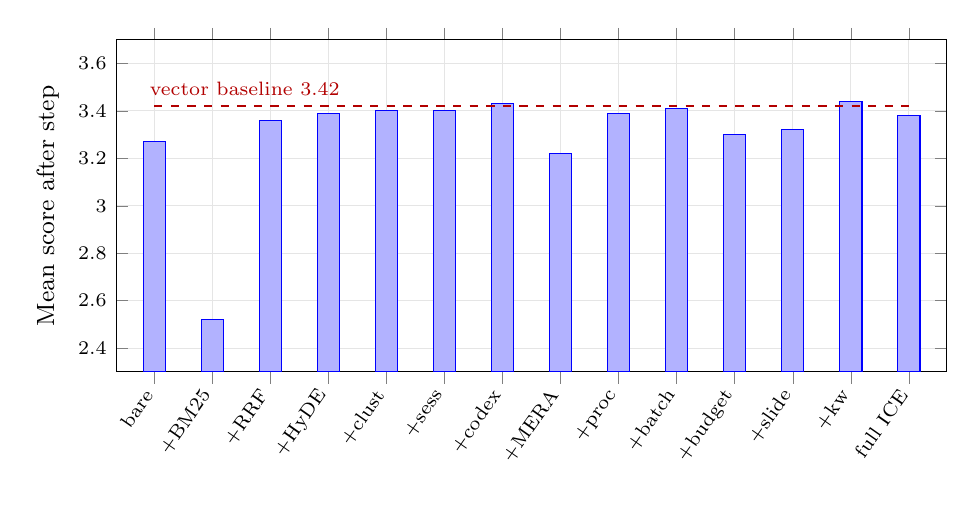
\begin{tikzpicture}
\begin{axis}[
    width=\columnwidth, height=5.8cm,
    ybar,
    bar width=8pt,
    ymin=2.3, ymax=3.7,
    ylabel={\small Mean score after step},
    ylabel near ticks,
    symbolic x coords={bare,+BM25,+RRF,+HyDE,+clust,+sess,+codex,+MERA,+proc,+batch,+budget,+slide,+kw,full ICE},
    xtick=data,
    x tick label style={rotate=55, anchor=east, font=\scriptsize},
    ytick={2.4,2.6,2.8,3.0,3.2,3.4,3.6},
    tick label style={font=\scriptsize},
    enlarge x limits=0.05,
    grid=major, grid style={gray!20},
    every axis plot/.append style={fill=blue!55!black, draw=blue!30!black},
]
\addplot coordinates {
 (bare,3.27) (+BM25,2.52) (+RRF,3.36) (+HyDE,3.39) (+clust,3.40)
 (+sess,3.40) (+codex,3.43) (+MERA,3.22) (+proc,3.39) (+batch,3.41)
 (+budget,3.30) (+slide,3.32) (+kw,3.44) (full ICE,3.38) };
\draw[dashed, red!70!black, thick] (axis cs:bare,3.42) -- (axis cs:full ICE,3.42)
  node[pos=0.12, above, font=\scriptsize, red!70!black] {vector baseline 3.42};
\end{axis}
\end{tikzpicture}
\caption{Feature ablation buildup (Dataset B, 67 probes). Each bar is the cumulative mean score after adding one feature to all previous ones. The only two movements clearing a paired bootstrap CI are the $+$BM25 drop and the $+$RRF recovery. The dashed line marks the single-leg vector baseline, which is not a buildup step; the full build finishes level with it.}
\label{fig:ablation-waterfall}
\end{figure}

\begin{table}[htbp]
\centering
\small
\caption{Recency effect by origin split (fact age). Probes grouped by the turn index at which they were created. Recency $\Delta$ is mean(late) $-$ mean(early). The fused configurations show positive recency---answers improve as the conversation grows---while the single-leg baseline is slightly negative.}
\label{tab:ablation-recency}
\begin{tabular}{@{}lrrrr@{}}
\toprule
\textbf{Condition} & \textbf{Early (0--400)} & \textbf{Mid (400--800)} & \textbf{Late (800--1200)} & \textbf{Recency $\Delta$} \\
\midrule
bare\_vector       & 3.00 & 2.83 & 3.42 & $+0.42$ \\
$+$BM25            & 2.20 & 3.05 & 2.49 & $+0.29$ \\
$+$RRF             & 3.00 & 2.83 & 3.54 & $+0.54$ \\
$+$keyword\_boost  & 2.90 & 3.28 & 3.60 & $+0.70$ \\
full\_ice          & 3.10 & 3.25 & 3.47 & $+0.37$ \\
vector\_baseline   & 3.50 & 3.15 & 3.47 & $-0.03$ \\
\bottomrule
\end{tabular}
\end{table}

\section{Experiment 2 Detailed Breakdowns}

\begin{table}[htbp]
\centering
\small
\caption{Evaluation metrics. Each is computed per probe and aggregated across the benchmark.}
\label{tab:metrics}
\begin{tabular}{@{}L{2.2cm}L{6.2cm}L{4.2cm}@{}}
\toprule
\textbf{Metric} & \textbf{Definition} & \textbf{What it measures} \\
\midrule
Score (1--5) & Mean absolute score from the judge & Answer quality \\
SPF & $\mathrm{mean\ score} / \mathrm{mean\ fragments}$ & Retrieval efficiency \\
TUR & $\mathrm{mean\ score} / (\mathrm{mean\ tokens}/1000)$ & Token efficiency \\
Win rate (\%) & Blind tournament: all four conditions' answers for a probe are anonymised, shuffled, and ranked best-to-worst in a single pass, independent of absolute scoring; the win rate is the share of appearances placed first & Relative preference, free of judge order bias \\
Hallucination (\%) & Share of probes where the judge detects information not present in the conversation & Faithfulness \\
Fragment count & Mean fragments injected per probe & Retrieval volume \\
Recency $\Delta$ & $\mathrm{mean\ score}(\mathrm{late\ bins}) - \mathrm{mean\ score}(\mathrm{early\ bins})$ & Longitudinal improvement \\
\bottomrule
\end{tabular}
\end{table}
\label{app:exp2-detail}

\begin{table}[htbp]
\centering
\small
\caption{Per-conversation breakdown (generalist conditions). ICE wins more head-to-head comparisons on every conversation. On Dataset A its win rate is more than double the baseline's.}
\label{tab:exp2-perconv}
\resizebox{\textwidth}{!}{%
\begin{tabular}{@{}lrrrrrr@{}}
\toprule
\textbf{Dataset} & \textbf{ICE score} & \textbf{Vec.\ score} & \textbf{ICE tok.} & \textbf{Vec.\ tok.} & \textbf{ICE win \%} & \textbf{Vec.\ win \%} \\
\midrule
A (Creative Writing)   & 3.63 & 3.50 & 19{,}434 & 24{,}360 & \textbf{37.2} & 18.0 \\
B (Long-Form Creative) & 4.28 & 4.33 & 24{,}108 & 21{,}257 & 32.8 & 22.9 \\
D (Academic Planning)  & \textbf{4.63} & 4.57 & 20{,}103 & 18{,}076 & 20.4 & 18.8 \\
\bottomrule
\end{tabular}%
}
\end{table}

Domain matters. On Dataset A (creative writing) ICE's win rate is more than double the baseline's. On Dataset B, the largest conversation at 1{,}119 turns, the baseline edges ahead on mean score (4.33 vs.\ 4.28) while ICE wins on win rate (32.8\% vs.\ 22.9\%) and uses 18\% more tokens serving more detailed answers. On Dataset D ICE wins on both.

\begin{table}[htbp]
\centering
\small
\caption{Score distribution (1{,}057 probes, Dataset C excluded). The mean-score tie masks a structural difference: ICE-MoE has the lowest score-1 rate but shifts mass from 5 to 3--4, producing lower-variance output.}
\label{tab:exp2-score-dist}
\begin{tabular}{@{}lrrrr@{}}
\toprule
\textbf{Score} & \textbf{ICE gen (\%)} & \textbf{ICE MoE (\%)} & \textbf{Vec.\ gen (\%)} & \textbf{Vec.\ MoE (\%)} \\
\midrule
1 (poor)       & 3.0 & 1.5 & 3.8 & 2.4 \\
2              & 5.9 & 4.3 & 4.3 & 3.9 \\
3 (acceptable) & 13.3 & 16.6 & 14.8 & 19.5 \\
4 (good)       & 18.1 & 19.7 & 17.2 & 16.3 \\
5 (excellent)  & 59.7 & 58.0 & 60.0 & 58.0 \\
\bottomrule
\end{tabular}
\end{table}

\begin{table}[htbp]
\centering
\small
\caption{Temporal score quality (1{,}057 probes, Dataset C excluded). Buckets: Good (4--5), OK (3), Poor (1--2).}
\label{tab:exp2-temporal}
\begin{tabular}{@{}lrrr@{}}
\toprule
\textbf{Condition} & \textbf{Good (4--5) \%} & \textbf{OK (3) \%} & \textbf{Poor (1--2) \%} \\
\midrule
Vector RAG generalist  & 77.2 & 14.8 & 8.0 \\
Vector RAG MoE         & 74.3 & 19.5 & 6.2 \\
Full ICE generalist    & \textbf{77.8} & 13.3 & 8.9 \\
Full ICE MoE           & 77.7 & 16.6 & 5.8 \\
\bottomrule
\end{tabular}
\end{table}

\section{Implementation Reference}
\label{app:implementation}

This appendix collects operational detail supporting Section~\ref{sec:architecture} but not required to follow the argument. A complete technical reference---the full training pipeline for the classifier and NER models, the controlled relation vocabulary in its entirety, GPU resource management, and the idempotency architecture---is the archived technical report in the repository, which describes the system at the tagged evaluation snapshot.

\subsection{Classification Engine}
\label{app:classifier}

The engine produces, per user turn, a set of topic tags, a set of intent tags, and one context-reliance label. These drive every downstream decision: which legs are weighted, how the budget is split, whether the wide-net fallback fires, and which model the router selects.

The learned head is deliberately tiny---a $384 \rightarrow 128 \rightarrow 25$ multi-layer perceptron with ReLU and 0.3 dropout. Its input is a single 384-dimensional embedding from a frozen \texttt{Qwen3-Embedding-0.6B} encoder; the shared linear head is sliced at inference into three blocks: 11 topic labels, 11 intent labels, and 3 context-reliance classes. Topic and intent decode multi-label (sigmoid, threshold 0.3, argmax fallback); context-reliance decodes single-label.

The rule-based pre-classifier computes five density signals in $[0,1]$ from the raw prompt---code density, sentiment density, meta density (references to the model itself), noise density, and reference density (anaphoric terms)---and evaluates five rules in order, returning the first that fires or none, in which case the learned head runs. The reference rule is special: it returns empty topic and intent tags but forces Long\_Term\_Memory, and the orchestrator then runs the head only to obtain topic and intent. A two-tier threshold on that rule (0.2 for short conversations, 0.1 past ten turns) is the engine's primary long-conversation memory bias.

\textbf{Override rules} run in evaluation order after either path: memory immutability, so once Long\_Term\_Memory is set nothing may downgrade it; a topic rule promoting creative turns to Long\_Term\_Memory; and a rule promoting technical turns containing anaphora. A second, API-level bias lives outside the classifier: past ten turns, or below 0.95 confidence, a Zero\_Shot label is upgraded before retrieval runs. Section~\ref{sec:limitations} discusses what this costs.

\textbf{Context-aware classification.} When a conversation ID is supplied, the learned path queries the last three episodic turns for that conversation (max 500 words), preferring summaries and falling back to the first 150 words of raw text, and prepends that context to the prompt before embedding.

\subsection{Codex Write Path and Retrieval}
\label{app:codex}

The graph spans four tables: entities (canonical name, aliases, properties JSONB, auto-regenerated context payload, embedding); edges (typed relations with strength, a confidence flag in \{pending, active\}, \texttt{valid\_from}, and \texttt{valid\_until}, where NULL means currently true); an append-only event log; and snapshots.

The triplet write path is the heart of temporal versioning. Entity resolution is two-stage---exact canonical-name match, then alias match, else create with a deterministic UUIDv5. The write branch then depends on the relation bucket: a property observation expires prior active edges of the same (source, relation) pair, writes a new edge, and overwrites the JSONB key; a reinforcement of an existing non-property edge increases strength and promotes from pending to active at strength $\geq 2$; a new relation between the same pair expires the old one only if the old relation is not multi-valued. Every state change emits an event, and the entity's context payload is rebuilt from the property map plus the ten most recent active outgoing edges. The event log is compacted by a worker that snapshots any entity exceeding 100 uncompacted events---textbook event sourcing, with the live edge table as current state, the log as audit trail, and snapshots as bounded replay.

\textbf{Micro-NER} is a BIO tagger (a $384 \rightarrow 128 \rightarrow 64 \rightarrow 3$ MLP over per-token embeddings). When the trained model is unavailable the system falls back to a capitalisation regex minus a stoplist; at the Experiment 2 snapshot the trained model was present and loaded. \textbf{Vector fuzzy matching} embeds the extracted entity strings, scans entity embeddings, and takes the best above a cosine threshold of 0.85---the mechanism that resolves a slightly misspelled proper noun to its canonical entity.

The retrieval leg extracts prompt entities, resolves them by fuzzy matching, optionally restricts to a conversation scope, and performs a BFS traversal to depth 3 over edges where \texttt{valid\_until IS NULL}, appending a labelled context payload per visited entity. \textbf{MERA}, the enumeration fallback for category queries, activates only when NER extracts no entities \emph{and} the prompt contains both a category trigger and an enumeration hint; candidates are deduplicated and ranked by 30-day mention count.

\subsection{Codex Limitations in Detail}
\label{app:codex-limits}

\textbf{The chunking paradox.} Extraction used 6{,}000-token chunks with 200-token overlap, chosen to avoid splitting sentences and to preserve narrative context. A 4B-parameter model does not have the effective reasoning capacity to process 6{,}000 tokens at once; beyond roughly 1{,}000--1{,}500 tokens attention dilutes, losing entities mentioned mid-chunk while over-weighting the beginning and end. Two failure modes follow: \emph{entity dropping}, where entities introduced mid-passage are never extracted, and \emph{relationship hallucination}, where subject and object of distant clauses are confused, producing syntactically valid but meaningless triplets. The right chunk size for a 4B extractor is closer to 512--800 tokens.

\textbf{Inert confidence and strength.} Edges carry a confidence flag and a decaying numeric strength, but both are under-used at retrieval time. Traversal follows any edge with \texttt{valid\_until IS NULL} regardless of either, and the only effect of an active confidence flag is a coarse $1.5\times$ fragment-level score boost. There is no reinforcement loop strengthening edges on retrieval, so frequently referenced facts do not rise in the ranking and traversal treats weak edges as equal to strong ones.

\textbf{Lexical versus semantic entity matching.} Retrieval resolves entities by canonical name or alias plus fuzzy matching over the context-payload embedding rather than the entity name. A user who establishes ``The Obsidian Citadel'' and later asks ``where is the main fortress located?'' gives the resolution step no lexical or embedded anchor for ``fortress,'' though a human reader resolves it immediately. This is a general limitation of entity-centric retrieval in free-form conversation: it assumes users refer to entities by canonical names or close aliases, which natural dialogue does not honour.

\subsection{Prompt Assembly}
\label{app:assembly}

The assembler emits a message list in a deliberately stable-prefix order to maximise cache reuse: (i)~a fixed system message with an inline persistent-context block rendering each active memory slot; (ii)~recent turns as alternating user/assistant pairs under dynamic per-turn word caps; (iii)~a single user message headed with the retrieved context, optionally tagged with cluster names when a cluster scope is populated; (iv)~a single assistant acknowledgement acting as a boundary marker, so the model treats the final user message as the live question rather than another history turn; and (v)~the live question. Because the system message, slots, and most of the recent-turn prefix change slowly, most of the prefix key/value tensors are in principle reusable across consecutive requests---though Section~\ref{sec:limitations} reports that the practical benefit is small.

A two-layer budget enforces final size: the orchestrator packs fragments to the retrieval token ceiling, then the API layer recomputes total words against a per-model ceiling (2{,}770 words for the deployed model) and iteratively pops procedural and episodic fragments until the budget is met, preserving document and graph fragments because they are the hardest to recompute and the most likely to carry the answer.

\textbf{Memory slots} are prepended verbatim to every prompt. Seven slot names are server-enforced: persona, user preferences, tool guidelines, project context, guidance, pending items, and session patterns. Slots are written through four paths: direct user update, batch initialisation, reflection-proposed but user-gated updates (high-stakes slots land in a review queue), and reflection-applied updates to pending items only.

\textbf{Context clusters} are conversation-scoped topical groupings. The centroid of member turn embeddings, renormalised to unit length after every change, is a 384-dimensional vector; membership is many-to-many. The clustering worker assigns each unassigned turn to the best existing cluster---combining embedding similarity, a bonus per shared entity, and tag overlap---or opens a new cluster when no candidate clears a 0.6 similarity threshold.

\subsection{Background Workers and Infrastructure}
\label{app:workers}

\begin{table}[htbp]
\centering
\small
\caption{Background workers. The cluster is self-maintaining: no operator intervention is required for the memory lifecycle.}
\label{tab:workers}
\begin{tabular}{@{}L{3.2cm}L{2.6cm}L{7.4cm}@{}}
\toprule
\textbf{Worker} & \textbf{Trigger} & \textbf{Function} \\
\midrule
Post-flight evaluator & every turn & lossless detection, summary, dispatch extractors \\
Codex extractor       & lossless turns  & triplet extraction and versioned writes \\
Procedural extractor  & every turn      & pattern detection, reinforcement or insertion \\
Episodic decay        & 1.5 h           & access-weighted decay, archive at 0.1, cold-store at 0.05 \\
Codex decay           & 1.5 h           & edge strength decay, demote below strength 0.3 \\
Procedural decay      & 1.5 h           & deactivation after 180 d with $<$ 3 reinforcements \\
Clustering            & 30 min          & assign unassigned turns, merge similar clusters \\
Reflection            & 2 h             & session synthesis, pattern crystallisation, slot proposals \\
Batch summariser      & 2 h             & 50-turn batches, preservation-prompt summaries \\
Sentinel monitor      & 30 min          & declarative rules: threshold, absence, and others \\
Fine-tune             & weekly          & retrain the classifier head on curated labels \\
Compaction            & manual          & snapshot entities with $\geq$ 100 uncompacted events \\
Drop zone             & filesystem      & ingest documents into the document store \\
Codex inject watcher  & filesystem      & ingest structured files into the graph with manual confidence \\
\bottomrule
\end{tabular}
\end{table}

All GPU-touching workers gate on a utilisation threshold polled from the driver and, in shared-model mode, additionally on a user-activity key with a short idle window. Retry countdowns are fixed per class. All workers are idempotent through a unique idempotency key, turning at-least-once delivery into effectively-once side effects.

The system is a single service exposing an OpenAI-compatible chat-completions endpoint plus routers for memory slots, user control, and the model registry, backed by PostgreSQL with pgvector---one 384-dimensional vector column per vector table, because the embedder is shared---and a worker fleet over a message broker. Configuration is a typed settings object read from the environment. Server-sent event types (\texttt{classified}, \texttt{retrieval}, \texttt{context\_ready}, \texttt{generating}, \texttt{degraded}) drive an observability panel and downstream monitoring. Classifier fine-tuning writes a timestamped checkpoint but does not auto-promote it, so production promotion requires a deliberate swap.

\end{document}
